%http://vim-latex.sourceforge.net/documentation/latex-suite.html#environment-mappings
%http://www.latextemplates.com/template/masters-doctoral-thesis
\documentclass[a4paper]{memoir}
\usepackage[utf8]{inputenc}
\usepackage{pgf}
\usepackage[margin=false,inline=true]{fixme}
\usepackage{listings} % DO NOT USE DRAFT DOCUMENT AS IT WILL NOT DISPLAY THE CODE
\usepackage{tikz}
\usetikzlibrary{arrows,automata,shapes}
\tikzstyle{block} = [rectangle, draw, fill=blue!20, 
    text width=5em, text centered, rounded corners, minimum height=4em]
\setcounter{secnumdepth}{3} 
\setcounter{tocdepth}{3} 


\fxsetup{theme=color}
\definecolor{fxnote}{rgb}{0.8000,0.0000,0.0000}
\author{Bauduin Raphaël}
\title{Oz Compiler}
\begin{document}
\newcommand{\nav}[1]{#1}
%\newcommand{\nav}[1]{}

% configure listings package to handle code as Oz code
%\lstset{language=Oz}
\lstset{language=Oz,basicstyle=\ttfamily\small,columns=fullflexible}

% requires memoir
% include git rev
\ifdraftdoc
\makeoddhead{plain}{}{}{\textit{Draft: \today{} Rev: \GITAbrHash{} \VCModifiedText{}}}{}
\fi

% write and require version control info
\immediate\write18{sh ./vc -m} 
%%% This file has been generated by the vc bundle for TeX.
%%% Do not edit this file!
%%%
%%% Define Git specific macros.
\gdef\GITHash{166c14995c66d3f18d28e1e99ea5e6f485604b6e}%
\gdef\GITAbrHash{166c149}%
\gdef\GITParentHashes{95e1d413565078e5f269c7f65b42db0ebcfaa4de}%
\gdef\GITAbrParentHashes{95e1d41}%
\gdef\GITAuthorName{Raphaël Bauduin}%
\gdef\GITAuthorEmail{rb@raphinou.com}%
\gdef\GITAuthorDate{2013-02-05 09:13:08 +0100}%
\gdef\GITCommitterName{Raphaël Bauduin}%
\gdef\GITCommitterEmail{rb@raphinou.com}%
\gdef\GITCommitterDate{2013-02-05 09:13:08 +0100}%
%%% Define generic version control macros.
\gdef\VCRevision{\GITAbrHash}%
\gdef\VCAuthor{\GITAuthorName}%
\gdef\VCDateRAW{2013-02-05}%
\gdef\VCDateISO{2013-02-05}%
\gdef\VCDateTEX{2013/02/05}%
\gdef\VCTime{09:13:08 +0100}%
\gdef\VCModifiedText{\textcolor{red}{with local modifications!}}%
%%% Assume clean working copy.
\gdef\VCModified{0}%
\gdef\VCRevisionMod{\VCRevision}%

\maketitle
\tableofcontents

%FIXME: add reference to next transformation for each node
%FIXME: add explanations of helper functions, like GetPos

\chapter{Introduction}
\section{Initial State}
A new virtual machine had been developed for Mozart2. The compiler
targeting the Mozart1 virtual machine had been adapted to target the new
virtual machine, and a boot compiler developed in Scala was used to compile it
for the new virtual machine.

This was seen as a temporary solution though, and a new compiler needed
to be developed. 


\section{Goal and Scope}
The new compiler was to be developed in Oz.
There were four goals set for the compiler:
\begin{enumerate}
  \item compile the whole language so that it can replace the current compiler in Mozart 2
  \item generate quality code, exploiting the capabilities of the virtual machine
  \item easy to understand and modular code
  \item the compiler should also be extensible so that, for example, support for a new instruction can be added without the recompilation of the compiler.
\end{enumerate}
Although the code is extensively commented, this report contributes to the third goal.

\chapter{Infrastructure}
\section{Virtual Machine}
The Mozart2 virtual machine was developed from scratch, with extensive additional support for the Oz language's concepts compared to the Mozart1 virtual machine. As a consequence, the code to be generated by the compiler should use these new capabilities and be different in some cases from the code generated by the Mozart1 compiler.


\subsection{Registers}\label{sec:intro:registers}
The Mozart2 virtual machine works with four types of registers. The description of the registers uses the concept of abstractions, which is precisely defined in the next section. It is however sufficient for the understanding of this section to equate the concept of abstraction with the concept of procedure.
\begin{description}
  \item[X registers]are work registers that should not be used to permanently
    store values. X registers are for example used to pass the arguments to calls. However, the values in these registers are lost after the call. %FIXME: isn't it X regs might be lost?
    %FIXME: combien de registres X disponibles,alloues?
  \item[Y registers]are locally persisting registers. They all have to be initialised at once at the start of an abstraction's code, before their use, which requires to know how many Y registers are needed.
  \item[G registers] are holding global variables, i.e. variables that are accessed by the abstraction, but that are not locally declared.
  \item[K registers] are holding constant values, be it integers, floats or records.
\end{description}

\subsection{Abstractions}\label{sec:vm:abstractions}
An Oz procedure is represented in the virtual machine by what is called an abstraction. An Oz program itself is implicitly placed in what is called a top level abstraction.
An abstraction holds references to G registers and to its code area. This code area has references to its K registers and the code itself. 

\begin{figure}[h]
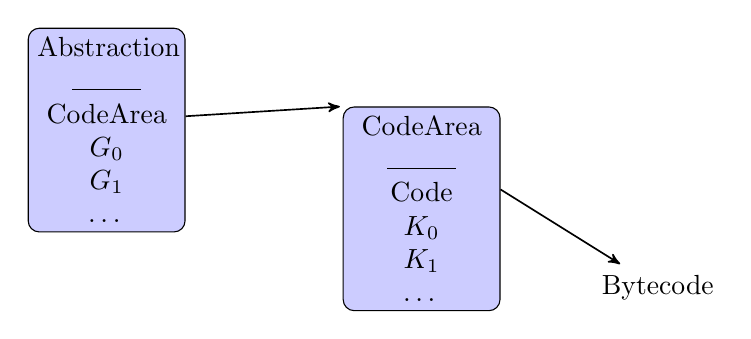
\begin{tikzpicture}[auto,every matrix/.style={ampersand replacement=\&,column sep=2cm,row sep=2cm},
                             to/.style={->,>=stealth',shorten >=1pt,semithick,font=\sffamily\footnotesize}]
  \node[block](abstraction) at (0,0) {Abstraction\\\line(1,0){25}\\
                             CodeArea\\
                             $G_0$\\
                             $G_1$\\
                             \dots\\};
  \node[block](codearea) at (4,-1) {CodeArea\\\line(1,0){25}\\
                             Code\\
                             $K_0$\\
                             $K_1$\\
                             \dots\\};
  \node[auto](bytecode) at (7,-2){Bytecode};

  \draw[to]  (abstraction.east)+(0,5pt) -- (codearea.north west);
  \draw[to]  (codearea.east)+(0,7pt)  --   (bytecode);
\end{tikzpicture}
\caption{Internals of the virtual machine}
\end{figure}
Capturing the global variables at the abstraction level is what provides
closures: a procedure captures the environment it was defined in.
The CodeArea is not stored in the abstraction itself, but is referenced from
it, simply because the same CodeArea can be referenced from multiple
abstractions. Let's illustrate this by an example. 

% reference: http://www.info.ucl.ac.be/~pvr/bookfigures/fig3_8.oz

\begin{lstlisting}
   fun {Sqrt X}
      fun {Improve Guess}
        (Guess + X/Guess) / 2.0
      end
      fun {GoodEnough Guess}
        {Abs X-Guess*Guess}/X < 0.00001
      end
      fun {SqrtIter Guess}
         if {GoodEnough Guess} then Guess
         else
            {SqrtIter {Improve Guess}}
         end
      end
      Guess=1.0
   in
      {SqrtIter Guess}
   end
\end{lstlisting}
The method Sqrt computes the square root by Newton's method. Each time Sqrt is
called, it defines three local functions. The two first reference the variable
X, which is a global variable for them, and which has probably a different
value at each call of Sqrt. However, the code area for each function is the
same for every call of Sqrt, and the virtual machine can simply create a new
abstraction with one global variable referencing the already existing code
area. 

If we have 2 simultaneous calls to Sqrt, for example {Sqrt 2} and {Sqrt 5}, we
would end up with this structure in the virtual machine:

\begin{verbatim}
Abstr1
CodeArea -------> CodeArea
G0=2          /   Code     -------------> Code
             /    K(2)                     with X registers
Abstr2      /
CodeArea --+
G0=5
\end{verbatim}

\begin{figure}[h]
  \centering
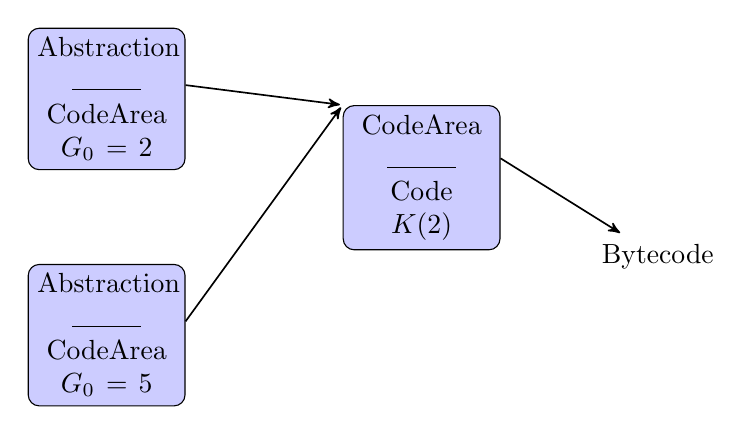
\begin{tikzpicture}[auto,every matrix/.style={ampersand replacement=\&,column sep=2cm,row sep=2cm},
                             to/.style={->,>=stealth',shorten >=1pt,semithick,font=\sffamily\footnotesize}]
  \node[block](abstraction) at (0,0) {Abstraction\\\line(1,0){25}\\
                             CodeArea\\
                             $G_0=2$\\
                             };
  \node[block](codearea) at (4,-1) {CodeArea\\\line(1,0){25}\\
                             Code\\
                             $K(2)$\\
                             };
  \node[auto](bytecode) at (7,-2){Bytecode};

  \node[block](abstraction2) at (0,-3) {Abstraction\\\line(1,0){25}\\
                             CodeArea\\
                             $G_0=5$\\
                             };

  \draw[to]  (abstraction.east)+(0,5pt) -- (codearea.north west);
  \draw[to]  (abstraction2.east)+(0,5pt) -- (codearea.north west);
  \draw[to]  (codearea.east)+(0,7pt)  --   (bytecode);
\end{tikzpicture}
\caption{Multiple Abstractions referring to the same CodeArea}
\end{figure}


\section{Target Language}
The compiler will have to generate code that can be passed to the assembler targeting the virtual machine. This assembler language has solid support for the virtual machine concepts as we'll see.
The assembler accepts an Oz list of instructions that are Oz records. 

\subsection{Register Operations}\label{sec:intro:opcode:registers}
Registers access instructions are proper to each type. To access the nth G X Y
registers, the instruction will respectively be \lstinline!g(n)!,
\lstinline!x(n)!, \lstinline!y(n)!. 

K registers are used to store constants, and are not numbered, but identified by
the value they store. The constant 2 will appear in the code as
\lstinline!k(2)!, the constant record \lstinline!r(a b c)! will appear in the
code as \lstinline!k(r(a b c))!.

As mentioned earlier, Y registers are persisting for the lifespan of the current frame. Their number has to be determined when the frame is initialised, and all needed Y registers are initialised at once with the instruction \lstinline!allocateY(n)! where n is the number of Y registers used in this frame.

X registers are work registers, and if a value in a X register needs to be accessed several time across calls, it has to be saved in a Y register. This is done with a move instruction: \lstinline!move(source_reg destination_reg)!.

%FIXME: what kind of registers can be unified. Does it make sense to unify X regs?
Unification is supported with the instruction unify(LHS RHS) where both LHS and RHS are registers.

\subsection{Jumps}\label{sec:opcode:jumps}
Code positions can be identified by labels, which need to be atoms or names. A label \lstinline!L! will appear in the code in a record \lstinline!lbl(L)!. 
Labels are required for jumps in the code. 
Jumps will move the execution to the label they have as argument. For example \lstinline!branch(endLabel)! will jump to the position in the code identified by the label \lstinline!endLabel!.

Conditional jumps will look at the value in a X register, and if this value is not true, it will jump to the code at the label it was given. That instruction also takes a label locating error handling code. Here is an example of conditional jump that will look at the value in X register 0: \lstinline!condBranch(x(0) elseLabel errorLabel)|!. If the value in x(0) is true, it continues execution. If it is false it jumps to the position in the code identified by the label \lstinline!elseLabel!. If an error occurs, it jumps to the label \lstinline!errorLabel!.


\subsection{Calls}\label{sec:opcode:calls}
%FIXME: can only call procedures and builtins?
Calls can be made with \lstinline!call(R Args)!, where R is a register identifying what to call (procedure or builtin) and Args is the number of arguments passed to the callee. The arguments of the call are not directly passed to the call instruction, but have to be placed in the X registers from 0 to Args-1 with move instructions before the call, as this is where the virtual machine will look for the arguments. The complete code for a call to a callee located in register Y 3 with three arguments which values come from Y registers 0 to 2 will thus be of the form:
\begin{lstlisting}
move(y(0) x(0))
move(y(1) x(1))
move(y(2) x(2))
call(y(3) 3)
\end{lstlisting}

A call done as last instruction of an abstraction should be made with the
\lstinline!tailCall! instruction, as this lets the virtual machine optimise the execution. It has the exact same specification as the call instruction, only the name of the instruction differs: \lstinline!tailCall(Callee Args)!.

\subsection{Records}\label{sec:opcode:records}
Records, tuples and cons are directly supported by the virtual machine, handling each of these particularly to ensure performance and efficiency.
A record of arity Arity, with NumberOfFeatures features is unified with register DestinationReg with this instruction:
\lstinline!createRecordUnify(k(Arity) NumberOfFeatures DestinationReg)!. which has to be followed by instructions to fill the features with their respective values:
\lstinline!arrayFill(Reg)! where Reg is the register corresponding to the feature's value.
The arity is supported by the virtual machine and includes the label and features without their respective values.

There are two special cases of records that are handled specifically by the virtual machine.
A con is a record with label '|' and with only 2 features numbers 1 and 2 and is initialised by
\lstinline!createConsUnify(DestinationReg)!. Again, this instruction has to be followed by arrayFill instructions, two in this particular case.
A tuple is a record with all numeric features. It is initialised by \lstinline!createTupleUnify(k(Label) NumberOfFeatures DestinationReg)! and followed by arrayFill instructions.
\subsection{Procedures}\label{sec:opcode:procedures}
A procedure is represented by what is called an abstractions (see Section \ref{sec:vm:abstractions}), which is created and stored in register DestinationReg with
\lstinline!createAbstractionUnify(k(CodeArea) GlobalsCount  DestinationReg)!
CodeArea is the assembled body of the procedure (see Section \ref{sec:codegen:procedures} for details). GlobalsCount identifies how many references to global variables this abstraction holds. It is the number of arrayFill instructions that will follow to initialise those global variables that the abstraction can access in G variables numbered from 0. The first arrayFill instruction will set the value of g(0), the second the value of g(1), \ldots

Here is code we will analyse:

\begin{lstlisting}
local
  A B P
in
  A=1           % in register X 0
  B=2           % in register X 1
  proc {P}      % in register Y 0
    {Show A+B}  % A and B are globals for P
  end           % access in g(0) and g(1) resp.
end
\end{lstlisting}

As noted in the code comments, we suppose, the compiler having done its work of registers assignation, variables A and B are stored in registers X 0 and 1 respectively, that the abstraction for procedure P is to be stored in register Y 0, and that P accesses to the value A and B via the register g(0) and g(1) respectively.
The body having been assembled and stored in the constant value CodeArea, this will lead to this code passed to the assembler:
\begin{lstlisting}
createAbstractionUnify(k(CodeArea) 2  y(0))
arrayFill(x(0))
arrayFill(x(1))
\end{lstlisting}

\subsection{Exceptions}
There is an opcode to setup an exception handler and jump to a label:
\begin{lstlisting}
  setupExceptionHandler(DestLabel)
\end{lstlisting}
If the code executed from \lstinline!DestLabel! raises an exception befire  the exception handler
is removed with \lstinline!popExceptionHandler!, the execution will jump to the
opcode following the instruction \lstinline!setupExceptionHandler!.

\section{Compiler input}\label{section:compilerinput}
%FIXME: add index for all record labels in the AST
The compiler takes as input the AST in the form of Oz records, and generates opcodes sent to the assembler. 
This section will present and describe the records received from the parser and
their corresponding Oz form.
Not all will be described here as an exhaustive list is available at %http://www.mozart-oz.org/home/doc/compiler/node7.html#appendix.syntax. 
\subsection{Position in source code}
Most records have the corresponding position in the source code available in their last feature, encoded in a record of the form \lstinline!pos(File Linebegin Columnbegin Fileend Lineend Columnend)!. This information has to trickle through all transformations so meaningful error messages can be given to the programmer in case of error.

For clarity and brevity, in the examples of AST included in this document, the positions will always be represented by the featureless record \lstinline!pos!. 
\subsection{Basic data types}
The basic data type described in this section are the simplest node found in the AST as they have no children and are the leafs of the tree.
These are the types that are currently handled, with their corresponding records in the AST:
\begin{description}
  \item[integers] fInt(Val Pos)
  \item[floats] fFloat(Val Pos)
  \item[atoms] fAtom(value position)
\end{description}

\subsection{Variables}\label{sec:input:variables}
A variable is found in a record fVar(VarName Pos)

\subsection{Unification}
A unification is found in a record fEq(LHS RHS Pos).
A=3 gives fEq(fVar(A \_) fInt(3 \_))

\subsection{Instructions sequence}
A sequence of instructions is wrapped in fAnd records, the first feature being usually one instruction, the second feature being a fAnd if more than one instruction follows,  or a single instruction. The code also handles the case when the two features are fAnd records. %FIXME: is this needed? 
Example:\\
\begin{tabular}{ p{0.3\textwidth} p{0.8\textwidth} }
  \begin{lstlisting}
    A=1
    B=2
    C=3
  \end{lstlisting}
&
  \footnotesize{
  \begin{verbatim}
  fAnd( fEq (fVar (A _) fInt (1 _))
        fAnd(fEq (fVar(B _)) fInt(2 _) 
             fEq(fVar(C _) fInt(3 _))))
  \end{verbatim}
  }
\end{tabular}

\subsection{Declarations}\label{sec:input:flocal}
Declarations are found in records of the form fLocal(Declarations Body Pos), where declarations and Body are both AST subtrees. 
For example:

\begin{lstlisting}
local
  A B C
in
  A=1
end
\end{lstlisting}
will give
\begin{verbatim}
fLocal(
       fAnd(
            fVar(A _) 
            fAnd(
                 fVar(B _) 
                 fVar(C _) 
                 _) 
            _) 
       fEq( 
            fVar(A _) 
            fInt(1 _) ))
\end{verbatim}

\subsection{Procedures}\label{sec:input:procedures}
\subsubsection{Definitions}
Procedures are found in records of the form \lstinline!fProc(Name Arguments Body Flags Pos)!, 
where the \lstinline!Arguments! and \lstinline!Body! features are AST subtrees. 
%FIXME: what can be Name? fVar, $. Other possibilities?
Example:

\subsubsection{Calls}
%FIXME: distinguish arguments and parameters?
Procedure calls are found in records of the form fApply(Proc Arguments Pos). 
Example:

\begin{lstlisting}
  {Compute 1 2 3}
\end{lstlisting}

will result in the AST portion:
\begin{lstlisting}
fApply(
       fVar(Compute _)
       |(fInt(1 _)
         |(fInt( 2 _)
           |fInt( 3 _))))
\end{lstlisting}

\subsection{Functions}\label{sec:input:functions}
Function definitions are found in the AST in fFun records, with the same features found in fProc records. Functions are simply procedures that implicitly return exactly one value. This similarity between functions and procedures can be seen in their similar AST for definitions and calls. This similarity will be exploited later on to merge both forms of AST into one.
However, only functions can be marked as lazy as in \lstinline!fun lazy {F N} .. end!. This lazy marker is translated in a flag.
\subsubsection{Definitions}
Function definitions are found in records fFun(Name Arguments Body Flags Pos). The features are identical to the procedure definition.
\subsubsection{Calls}
The calls of functions are identical to the call of procedures as they are found in fApply.
\subsection{Arithmetic operators}\label{sec:input:operators}
Arithmetic operators are parsed as records of the form fOpApply(Operator Args Pos), which first feature is the operator to apply, and its second feature being the list of operands. It also has a position record as third feature. For example
\lstinline!5+2! is parsed as:
\begin{lstlisting}
      fOpApply(
         '+'
         |(
            fInt(5 pos)
            |(
               fInt(2 pos )
               
            )
         )
         pos
      )

\end{lstlisting}
\subsection{Nesting marker \$}\label{sec:input:nestingmarker}
In Oz, some statements can be transformed in expressions by the use of the \$ marker. This marker is found in the AST as a record fDollar() with a unique feature: it position.
The statements that can be transformed in expressions are
\begin{itemize}
  \item Function, Procedure, Functor and Class declarations. For example
    \lstinline!X=fun{\$ A B} .. end!
  \item In the parameters list of a call to a procedure, in the location of an
    expression. For example \lstinline!{Foo A..\$..N}!
  \item In a pattern position of a parameter of a call. For example
    \lstinline[mathescape]!{Foo bar(A..$\$$..N) baz}!
\end{itemize}
Note that although functions can unify their parameters with values, like in 
\begin{lstlisting}
  fun {F A ?R2}
     R2=3*A
     2*A
  end
\end{lstlisting}
It makes absolutely no sense to put a nesting marker as second argument to a call of this function, like in 
\lstinline[mathescape]!{F 2 $\$$}! because the call itself is already an expression.


\subsection{Cells}\label{sec:input:cells}
\subsubsection{Assignation}
fColonEquals(Cell Val Pos) %FIXME
\subsubsection{Read}
fAt(Cell Pos) % FIXME
\subsection{Records}\label{sec:input:records}
Without describing the whole syntax, here is a reminder of the record syntax in Oz code. A record is refined by \lstinline!Label(F1:V1 F2:V2)! where the label and features ($F_i$) can be an atom or a variable, and the values ($V_i$) can in addition to this be the result of a function call. Features can be left out, in which case they are implicitly assigned increasing values from 1.

Records are present in the AST in records with label fRecord. Its label is the first feature, and the second feature is the list of feature/value pairs. If no feature was specified, the entry in the list is simply the value. If a feature was specified, the entry in the list is a record fColon, with the first feature being the feature and second feature being the value. All this will become much clearer with the following examples.

Here is the AST corresponding to the record definition \lstinline!rec(f1:v1 f2:v2)!. We see that the label (rec) is an atom located in an fAtom record. The pairs of features and their respective values are wrapped in fColon.

\begin{lstlisting}
   fRecord(
      fAtom(rec pos)
      |(
         fColon(
            fAtom(f1 pos)
            fAtom(v1 pos)
         )
         |(
            fColon(
               fAtom(f2 pos)
               fAtom(v2 pos)
            )
            nil
         )
      )
   )
\end{lstlisting}

When the feature is not explicitly given, the item in the list of features and their respective values is simply the value. Here is the AST of this record \lstinline!rec(v1 f2:V2)!. The first item in the list is simply an atom, the value of the first feature. Note that the value of the feature f2 is a variable in this case.

\begin{lstlisting}
   fRecord(
      fAtom(rec pos)
      |(
         fAtom(v1 pos)
         |(
            fColon(
               fAtom(f2 pos)
               fVar(V2 pos)
            )
            nil
         )
      )
   )
\end{lstlisting}


\subsection{Wildcards}\label{sec:input:wildcard}
Oz syntax allows to put a wildcard \lstinline!_! in the location of a value we want to ignore, for example in calls and records pattern matching. These markers are present in the AST in the form of a record \lstinline!fWildcard(Pos)!.
Ignoring the value returned by a function is thus written \lstinline!_={F N}!. 
This allows the user to not declare variables he wouldn't use anyway, which would in addition raise a warning about a variable used only once\ldots

Pattern matching is covered extensively in Section \ref{sec:input:patternmatching}.

\subsection{Threads}
Thread instructions are present in the AST in the form of records with label fThread, and with two features: the body of the thread, and its position in the source code:
\begin{lstlisting}
   thread Body end
\end{lstlisting}
results in
\begin{lstlisting}
   fThread(Body pos)
\end{lstlisting}
\subsection{Locks}\label{sec:input:locks}
Oz enables the programmer to protect a critical section with a lock previously create with \lstinline!L={NewLock}!:
\begin{lstlisting}
   lock L then
      % critical section
   end
\end{lstlisting}

This code results in a fLockThen record in the AST, with 3 features: the lock L,
the body of the critical section, and the position in the code:
\lstinline!fLock(L Body Pos)!.
\subsection{If then else}
The if..then..else construct is put in records:
fBoolCase( Condition ThenCode ElseCode)
The else part is optional in Oz. In this case, ElseCode is a record \lstinline!fNoElse(pos)! in the AST.
\subsection{Boolean combinations}\label{sec:input:booleancombinations}
The boolean conjunction operation in Oz represented by the keyword \lstinline!andthen!. Such a conjunction is present in the AST in the form of a record \lstinline!fAndThen(First Second)!, where first and second must be expressions with a boolean value.
The boolean disjunction operation is done thanks to the keyword \lstinline!orelse!, present in the AST in the form of a record \lstinline!fOrElse(First Second)!.
\subsection{Case Instruction and Pattern Matching}\label{sec:input:patternmatching}
The Case instruction in Oz is of the following form where optional parts are enclosed in double square brackets ([[ ]]).
\begin{lstlisting}
   case Value                           % _
   of Pattern1 [[andthen Guards1]] then %  \____ This is a clause
     Code1                              % _/
   [] Pattern2 [[andthen Guards2]] then
     Code2
   ..
   [[else
     ElseCode]]
   end
\end{lstlisting}
This ends up in the AST in a record of the form \lstinline!fCase(Value Clauses ElseCode pos)!.
\lstinline!Clauses! is a list of records each representing one clause and containing the clause' pattern, guards and code. We will analyse these further below.
The else part of the instruction is optional. If no else is provided, then ElseCode in the AST is a record \lstinline!fNoElse(pos)!.

A clause with no guards is present in the AST in the form of a record \lstinline!fCaseClause(Pattern Body)!. \lstinline!Pattern! can be a constant value (integer, string, record, \ldots), present in the AST as described earlier. It can also be a record where a feature value is not a constant but a variable (in a \lstinline!fVar(Name pos)! record as described in section \ref{sec:input:variables}). In case of a match of the constant feature values in the pattern, this declares said variable and assigns the value of the corresponding feature in the value the pattern is tested against. Here is an example:
\begin{lstlisting}
  R=lab(a b c d)
  case R
  of lab(a B c d) then
    {Show B}  % B's value is b
  end
\end{lstlisting}
Features of a record in a pattern can also have the wildcard \lstinline!_! as value, represented in the AST as described in section \ref{sec:input:wildcard}.

The pattern can also be or contain an open record specifying only the first features which should match, as in the following example:
\begin{lstlisting}
  R=lab(a b c d)
  case R
  of lab(a b ...) then
    % Code for record with label lab
    % and value a and b for two first features.
  end
\end{lstlisting}
The syntax for an open record pattern is the same as for a record pattern, except that subsequent features that should be ignored are replaced by \lstinline!...!. Also in the AST an open record is very similar to a record. Only the label changes to \lstinline!fOpenRecord!, and only the specified features are present in the AST, the \lstinline!...! being absent from the AST. Here is an example of an open record:
\lstinline!lab(a b ...)! 
and its AST representation:
\begin{lstlisting}
   fOpenRecord(
      fConst(lab pos)
      |(
         fColon(
            fConst(1 pos)
            fConst(a pos)
         )
         |(
            fColon(
               fConst(2 pos)
               fConst(b pos)
            )
            nil
         )
      )
   )
\end{lstlisting}

Records and open records can of course be nested.

A clause with guards is present in the AST in the form of a record \lstinline!fSideCondition(Pattern Decls Guards Pos)!, where \lstinline!Pattern! is as above, Decls is usually skipped (\lstinline!fSkip(pos)!)%FIXME: what are decls??
and Guards is simply the AST of the code of the guard (without the \lstinline!andthen! introducing the guard).
Guards must be an expression with a boolean value, possibly using the boolean combinations of section \ref{sec:input:booleancombinations}.

Variables can also be used in patterns for their value, and not as a new capture
declaration. This is done by prefixing the variable with an exclamation mark.
Here is an example:

\begin{lstlisting}
A=a
case V
of rec(A b c) then
   % matches rec(_ b c), i.e. all records with label rec, second feature value
   % b, third value c, with A being a new capture variable
[] rec(!A b c) then
   % only matches rect(a b c)
end
\end{lstlisting}

and escaped variable ends up in the AST as wrapped in an \lstinline!fEscape!
record. \lstinline!A! appears in the AST as \lstinline!fEscape( fVar(A pos) pos)!.
\nav{The next transformation of \lstinline!fEscape! nodes is done by the Namer,
see Section \ref{sec:arch:namer:patternmatching}.}

Oz pattern matching also support what is called pattern conjunction, enabling to assign the value of a subexpression of the pattern to a variable. It is better illustrated by an example:
\begin{lstlisting}
   case V 
   of rec(V=inner(a b ...)) then
   ...
   end
\end{lstlisting}

In the clause'code, the variable V will have the value of the inner record.
These pattern conjunctions are present in the AST in \lstinline!fEq! record just 
like unification instructions.
Note that just like unifications (and unlike \lstinline!local..in..end!), the variable implicitly declared can be at the
left as well as at the right side of the equal sign. So the pattern
\lstinline!rec(V=inner(a b ...))! is equivalent to \lstinline!rec(inner(a b ...)=V)!


\subsection{Classes}
Let's illustrated the AST we get for a class definition with an example:

\begin{lstlisting}
   class C
      meth init skip end
      meth hello(A1)
         {Show 'hello'}
         {Show A1}
      end
   end
\end{lstlisting}
which results in this AST:
\begin{lstlisting}

   fClass(
      fVar('C' pos )
      nil
      |(
         fMeth(
            fAtom(init pos )
            fSkip(pos )
            pos)
         |(
            fMeth(
               fRecord(
                  fAtom(hello pos )
                  |(
                     fMethArg(
                        fVar('A1' pos )
                        fNoDefault)
                     nil))
               fAnd(
                  fApply(
                     fVar('Show' pos )
                     |(
                        fAtom(hello pos )
                        nil)
                     pos)
                  fApply(
                     fVar('Show' pos )
                     |(
                        fVar('A1' pos )
                        nil)
                     pos))
               pos)
            nil))
      pos)
\end{lstlisting}

We see that class definitions are found in 
\lstinline!fClass(ClassVar SpecsList MethodsList Pos)!.
A method is found in records \lstinline!fMeth(Signature Body Pos)!.
For methods without argument, \lstinline!Signature! is simply the method name.
In the example, this is illustrated by the \lstinline!init! method.
For methods with arguments, \lstinline!Signature! is the AST of a record which label is the method name, and the
values in the record are the method arguments found in 
\lstinline!fMethArg(Var DefaultValue)!, where \lstinline!DefaultValue! is
\lstinline!fNoDefault! if none was provided.
This is illustrated by the method \lstinline!hello(A1)!.

The class of this example had no feature, attribute, parent or property defined, hence the empty
list as second value in the record.
Both attribute and features are placed in this list. Attributes are placed in
\lstinline!fAttr(AttrsList)! records and features are placed in
\lstinline!fFeat(FeatsList)! records. Both these records have one feature which
value is a list. Each attribute and feature corresponds to one item in its
respective list. If the attribute or feature has a default value, its
corresponding item is a record with label \lstinline!'#'! and two values: the
first is the name of the attribute or feature, the second is the default value.
If no default value is defined, the item in the list is simply the name of the
attribute or the feature.
Let's look at an example. A class with the following attributes and feature
definition
\begin{lstlisting}
      attr
         count:0
         state
      feat
         type:repeater
  
\end{lstlisting}
will have its list of attributes and features looking like this:
\begin{lstlisting}
      |(
         fAttr(
            |(
               #(
                  fAtom(count pos )
                  fInt(0 pos ))
               |(
                  fAtom(state pos )
                  nil))
            pos)
         |(
            fFeat(
               |(
                  #(
                     fAtom(type pos )
                     fAtom(repeater pos ))
                  nil)
               pos)
            nil))
\end{lstlisting}
We see that the \lstinline!count! attribute is placed in a '\#' record, but not
the \lstinline!state! attribute.
We also see clearly that all attributes are placed in one \lstinline!fAttr!
record, and all features in on \lstinline!fFeat! record.

This list also contains more information: the parents of the class, as well as
the properties of the class. 

The parents are located in \lstinline!fFrom(ParentsList)!. 
Here is an example from a class inheriting from classes \lstinline!A! and
\lstinline!B!. In Oz, this class will be defined by
\begin{lstlisting}
  class C from A B
    ..
  end
\end{lstlisting}
and this will result in this element in the list
\begin{lstlisting}
           fFrom(
            |(
               fVar('A' pos )
               |(
                  fVar('B' pos )
                  nil))
            pos)
\end{lstlisting}

The properties of a class are also present in that list, under \lstinline!fProp!
records. A class having the locking property would have this \lstinline!fProp! record:

\begin{lstlisting}
           fProp(
               |(
                  fAtom(locking pos )
                  nil)
               pos)
\end{lstlisting}

When a class has the \lstinline!locking! property, a lock is implicitly created,
that can be used in a method with the \lstinline!lock! statement without
specifying the lock object, as this:

\begin{lstlisting}
   meth update(A)
      lock
         ..
      end
   end
\end{lstlisting}

This \lstinline!lock! instruction is put in the AST as a node
\lstinline!fLock(Body Pos)!. The next transformation to this node 
takes place in the desugar step described page \pageref{desugar:classes:lock}.

Assignation to attributes can be done in two ways. The first has the same syntax
as cell updates, described in Section \ref{sec:input:cells}:
\begin{lstlisting}
  my_attr:=NewVal
\end{lstlisting}
and is found in the AST just as a cell update operation under a node
\lstinline!fColonEquals!.

The second uses the syntax \lstinline!<-!:
\begin{lstlisting}
  my_attr<-NewVal
\end{lstlisting}
and is found in the AST under a node \lstinline!fAssign(LHS RHS pos)!.

\label{compilerinput:classes:headcapture}The method head can also be captured and made available to its body,as in 
\begin{lstlisting}
   meth echo(First ...)=H
      Body
   end  
\end{lstlisting}
At run time, the H variable will give access to the message sent to the object, with the actual arguments list.
\begin{lstlisting}
               fMeth(
                  fEq(
                     fOpenRecord(
                        fAtom(echo pos )
                        |(
                           fMethArg(
                              fVar('First' pos )
                              fNoDefault)
                           nil))
                     fVar('H' pos )
                     pos)
                  BodyAST
                  Pos)
\end{lstlisting}

Method can also be defined as private by using a variable name as their label:
\begin{lstlisting}
   meth A(V)
      Body
   end
\end{lstlisting}
resulting in the AST

\begin{lstlisting}
   fMeth(
      fRecord(
         fVar('A' pos )
         |(
            fMethArg(
               fVar('V' pos )
               fNoDefault)
            nil))
      BodyAST
      pos)
\end{lstlisting}
The method \lstinline!A! will be bound to a new name, only visible in the class
definition's scope (see Section \ref{sec:arch:namer:classes} for details).

Method can also have dynamic labels assigned, by escaping the variable holding
the label to use:
\begin{lstlisting}
  meth !A(V)
     Body
  end
\end{lstlisting}
which results in the AST:
\begin{lstlisting}
    fMeth(
       fRecord(
          fEscape(
             fVar('A' pos)
             pos)
          |(
             fMethArg(
                fVar('V' pos)
                fNoDefault)
             nil))
       BodyAST
       pos)

\end{lstlisting}

\subsection{Loops}
There are three forms of the \lstinline!for..in..do..end! statement, working
respectively on list, ranges, and C-like for loops conditions.
\subsubsection{Iterating over lists}
The Oz syntax is best illustrated by an example:
\begin{lstlisting}
   for Var in L do {Show Var} end
\end{lstlisting}
\lstinline!Var! is bound to each element of L in turn, and the code executed.
Hence this code will show all elements of the list L.

Multiple list can be iterated:
\begin{lstlisting}
   for I in L J in L2 do {Show I#J} end
\end{lstlisting}
but note that both lists are iterated in parallel, and the loop ends once the
end of one of the list is reached. The number of time the body of the loop is
called is thus the number of elements of the smallest list.

The AST of the first \lstinline!for! example is:
\begin{lstlisting}
   fFOR(
      |(
         forPattern(
            fVar('Var' pos )
            forGeneratorList(
               fVar('L' pos )))
         nil
      )
      fApply(
         fVar('Show' pos )
         |(
            fVar('Var' pos )
            nil)
         pos)
      pos)
\end{lstlisting}

The first value in the \lstinline!fFor! record is the list of patterns, one
for each list. Each item of this list is a \lstinline!forPattern! record, with
its first value being the variable that will be available in the loop, and the
second value an \lstinline!fGeneratorList! record referencing the list over which to
iterate.
The second value in the \lstinline!fFor! record is the code to be executed for
each element of the list.

\subsubsection{Iterating over ranges}
Here is an example of a \lstinline!for! loop iterating over integers from 1 to 5
with a step of 2, resulting the execution of the body of the loop for integers 1
3 and 5:
\begin{lstlisting}
   for I in 1..5;2 do {Show I} end
\end{lstlisting}

\begin{lstlisting}
   fFOR(
      |(
         forPattern(
            fVar('I' pos )
            forGeneratorInt(
               fInt(1 pos )
               fInt(5 pos )
               fInt(2 pos )))
         nil)
      fApply(
         fVar('Show' pos )
         |(
            fVar('I' pos )
            nil)
         pos)
      pos)
\end{lstlisting}

The AST is very similar to the first loop form, only the
\lstinline!fGeneratorList! record is replaced by a \lstinline!forGeneratorInt!
record holding the specification of the range and step to use.

\subsubsection{C-style for loops}
Iterating over integers from 1 to 5 with a step of 2 can also be written in the C-style for loop:
\begin{lstlisting}
   for I in  1;I<4;I+1 do  {Show I} end
\end{lstlisting}
It takes a generator comprised of 3 expressions: \lstinline!E1;E2;E3! where
\lstinline!E1! is the start value, \lstinline!E2! is the test condition, the
looping continuing as long at it evaluates to true, and \lstinline!E3! is the
next value's expression.
It is found in the AST as:
\begin{lstlisting}
fFOR(
      |(
         forPattern(
            fVar('I' pos )
            forGeneratorC(
               fInt(1 pos )
               fOpApply(
                  '<'
                  |(
                     fVar('I' pos )
                     |(
                        fInt(4 pos )
                        nil))
                  pos)
               fOpApply(
                  '+'
                  |(
                     fVar('I' pos )
                     |(
                        fInt(1 pos )
                        nil))
                  pos)))
         nil)
      fApply(
         fVar('Show' pos )
         |(
            fVar('I' pos )
            nil)
         pos)
      pos)
  
\end{lstlisting}

The notable difference is the generator record now being
\lstinline!forGeneratorC! holding the three expressions.

\subsection{Exceptions}\label{sec:input:exceptions}
An exception can be raised with the instruction \lstinline!raise E end!, where
\lstinline!E! is a record value. %FIXME: is an exception always a record?
A raise instruction is found in the AST under a node \lstinline!fRaise(E pos)!.
\nav{Its next transformation takes place in the desugar step (see Section
\ref{sec:arch:desugar:exceptions}).}

Code possibly raising exceptions can be wrapped in a try-catch-finally
instruction of this form:
\begin{lstlisting}
   try Code
   catch
      Pat1 then
      Code1
   [] Pat2 then
      Code2
   finally
      FinalCode
   end
\end{lstlisting}

We can see that the catch part specifies multiple clauses each with a pattern
against which the exception raised will be tested, and code which will be
executed if the pattern effectively matched. \lstinline!finally! introduces code
that will be executed in all cases after \lstinline!Code! and the possible
matching catch clause.

It results in this AST:
\begin{lstlisting}
   fTry(
      Body
      fCatch(
         |(
            fCaseClause(
               Pat1
               Code1)
            |(
               fCaseClause(
                  Pat2
                  Code2)
               nil))
         pos)
      FinalCode
      pos)
\end{lstlisting}

which exactly mirrors the Oz code: \lstinline!fTry! holds the AST of the body,
which is code possibly throwing an exception, the \lstinline!fCatch! record containing the list of
clauses, and the \lstinline!finally! code. The \lstinline!finally! may be left
out of the Oz code, in which case \lstinline!FinalCode! is the record
\lstinline!fNoFinally!.
Clauses of a catch are present in the AST in the same form as clauses of a case
instruction (see Section \ref{sec:input:patternmatching}), i.e. a
\lstinline!fCaseClause! record holding the pattern and the code to execute if
the pattern matches. This similarity will be exploited by the compiler, notably
in the namer, which is the next transformation to be applied to an
\lstinline!fTry! node (see Section \ref{sec:arch:namer:exceptions}).
\subsection{Arrays}
A special notation is available for assigning value to arrays, as to mimic the
matrix notation. As such, the code \lstinline!A.I:=V! will assign \lstinline!V!
to the \lstinline!I!th element in the array \lstinline!A!.
This results in node \lstinline!fDotAssign! in the AST. The node generated by
the parser is
\begin{lstlisting}
   fDotAssign(fOpApply('.' [A I] Pos1) 
              V 
              Pos2) 
\end{lstlisting}
The first transformation applied to these nodes takes place in the desugar step,
described in Section \ref{sec:arch:desugar:dotassign}.
\chapter{Compiler}
\section{Architecture}
The AST received from the parser goes through several transformations. These transformations are implemented by functions taking as only argument the AST, and they return the transformed AST.
These functions all have the same structure:
\begin{figure}[h]
\begin{lstlisting}
   fun {Transform AST}
      fun {TransformInt AST Params}
         case AST
         of ... then
         else
            {DefaultPass AST TransformInt Params}
         end
      end
      InitialParams = ...
   in
      {TransformInt AST InitialParams}
   end
\end{lstlisting}
\caption{Structure of a transformation function}
\end{figure}
Having the same structure enables the use of the function \lstinline!DefaultPass!, which calls the function passed as second arguments recursively on the AST with \lstinline!Params! as last argument, but returns the AST unchanged. This facilitates the recursive calls for default behaviour on elements not modified by the transformation.
Params is a record with label \lstinline!params!, and features are added
according to use. For example, this \lstinline!Params! argument is used by
the \lstinline!Globaliser! described in Section \ref{sec:arch:globaliser}. All
passes take a Params as last argument, even if some do not use it. 
% Should I add that fAnd takes a pos feature and fAndThen not, and that I had to
% tweak the function WrapIn as a consequence?


Although all passes work exclusively on the AST, the transformations described in later sections can and will often be illustrated more clearly and concisely by giving the Oz code corresponding to the ASTs before and after the transformation. 

\subsection{Declarations Flattener}\label{sec:arch:declsflattener}
The Oz language accepts complex instructions in the declaration part of \lstinline!local Decls in Body end!. This brings the need to decide what variables are declared for each instruction present in the \lstinline!Decls!. 
For example, in unification, only the left hand side variable gets declared, and only B is implicitly declared in the following code snippet:
\begin{lstlisting}
   local
      B=2*A
   in
      ...
   end
\end{lstlisting}
Luckily, this has been clearly formalised by the Oz implementers and published on the web\footnote[]{http://www.mozart-oz.org/documentation/notation/node6.html}. This information has been included in Appendix \ref{appendix:patternvariables}. The namer simply applies these rules to move all code to the \lstinline!Body! beginning, keeping only simple variable declarations in \lstinline!Decls!.

\subsection{Namer}\label{sec:arch:namer}
%FIXME: add fFOR
The namer  basically replaces all occurrences of a variable's \lstinline!fVar! by \lstinline!fSym! records holding a symbol instance representing said variable. All uses of a variables are replaced by the same symbol instance. This symbol holds information about the variable, that will be completed by subsequent compiler passes, such as the type of the symbol, its allocated register,\ldots and is documented in Appendix \ref{appendix:symbol}.

In declarations, the namer creates a new symbol for the declared variables, in other code, it looks at already defined symbols and replaces \lstinline!fVar!s by a \lstinline!fSym! record containing the existing symbol for that variable. This works because a variable can only be used after it has been declared. The namer can thus be sure to find a symbol for variables it encounters in the AST, or it is an error.

The \lstinline!Namer! also has some work to do on patterns and the variables it
implicitly declares. As a consequence, it also handles and transforms the AST
for functions and procedures.

The set of maps from a variable name to its corresponding symbol is called environment, and is maintained by the namer.


\subsubsection{Declarations}
So the question raises of when do variables get declared.
One such construct is of course the explicit declaration instruction \lstinline!local Decls in Body end!, present in the AST in the form of \lstinline!fLocal! records introduced in section \ref{sec:input:flocal}. At this stage, \lstinline!Decls! only contains simple variables declaration, thanks to the declaration flattener (see Section \ref{sec:arch:declsflattener}). \lstinline!fLocal! introduces a new environment, in which the variables declared in its first feature are added to the environment of the code present in its second feature, possibly erasing mappings for variables with the same name coming from the parent environment. 

Another kind of declaration is found in the definition of procedures and functions. Indeed, fProc (section \ref{sec:input:procedures} and fFun (section \ref{sec:input:functions}) records also implicitly declare the variables for their formal parameters. % see test 029

Still another kind of declaration happens in pattern matching (section \ref{sec:input:patternmatching}), when a record present in the pattern has a feature that is a variable. This case is analysed specifically in section\ref{sec:arch:namer:patternmatching}.

These variables get implicitly declared and added to the environment in which not only the clause' body but also its guards will be executed.


It is these manipulations of the environments that make that the code in Figure~\ref{fig:namer_nested_locals} does not throws an error of impossible unification of A with 6. Indeed, the inner variable A gets another symbol assigned than the outer one, and replaces it in the environment of the inner instructions. Thus there is no ambiguity in the \lstinline!Show! instruction as to which its argument is, and it effectively shows 6.
\begin{figure}
\begin{lstlisting}
local
   A=5
in
   local 
      A=6
   in
      {Show A}
   end
end
\end{lstlisting}
\caption{Nested locals handled by Namer}
\label{fig:namer_nested_locals}
\end{figure}


\subsubsection{Non-declaration code}
In code not declaring variables, the namer's job is much simpler: it will simply
replace all occurrences of fVar records by a fSym record having the corresponding symbol as first feature.
\subsubsection{Case Pattern Matching}\label{sec:arch:namer:patternmatching}
For pattern matching with the \lstinline!case! instruction the namer will have
more work to do, which we will discuss now. Let's note
\lstinline!PatternX(Var1,Var2,..)! the pattern identified by X and implicitly
declaring variables \lstinline!Var1!,\lstinline!Var2!,\ldots, and let's use the same convention for code fragments \lstinline!CodeX(Var1,Var2,..)! and guards \lstinline!GuardsX(Var1,Var2,..)! using those implicitly declared variables.

The transformation of the AST corresponding this Oz code:
\begin{lstlisting}
case Val
of Pattern1(A,B) andthen Guards1(A) then
   Code1(A,B)
[] Pattern2(B,C) andthen Guards2(C) then
   Code2(B,C)
else
   ElseCode
end
\end{lstlisting}
results in an AST corresponding to this Oz code:
\begin{lstlisting}
local
  A1 B1 B2 C2
in
   case Val
   of Pattern1(A1,B1) andthen Guards1(A1) then
      Code1(A1,B1)
   [] Pattern2(B2,C2) andthen Guards2(C2) then
      Code2(B2,C2)
   else
      ElseCode
   end
end
\end{lstlisting}

Here is the way how it is achieved. The compiler traverses each clause in turn,
and collects all symbols introduced during this operation. It creates a new
environment for this clause, which is updated with captures done in the
pattern. After that, the namer traverses the ASTs of the Guards and the Code
using this updated environment. and restores the original environment, on which
the next clause will build its own environment. This shows clearly that
although all capture variables are are technically reachable from all clauses'
bodies, it will never be the case as the environment on which a clause builds
its own is the environment of the case instruction, not the environment updated
by the previous clause. 
%FIXME: add reference and detailed description of secure storage

In addition, the \lstinline!fSym! record corresponding to these capture
variables are themselves stored in an unforgeable secure structure (as
described in CTMCP Section 3.7.5) which is itself wrapped in an
\lstinline!fConst!. The reason of this manipulation is to prevent manipulations
of those symbols by later compiler passes. Now these will be handled as
constants in all subsequent compiler passes. Another consequence of this is
that the records implicitly declaring variables in a pattern are seen as
constant records, all features being constants! And these are treated as such,
notably in the desugaring of records (section \ref{sec:arch:desugar:records}).

To ease the work of future passes and improve readability of their code, the
namer also replaces \lstinline!fEq! records of pattern conjunctions in
\lstinline!fPatMatConjunction! records.

Patterns with guards require some additional work. These are present in the AST
as \lstinline!fSideCondition(Pattern Decls Guards Pos)!. First, a new symbol is
introduced and unified with the \lstinline!Guards! expression. The record in the
AST is replaced by \lstinline!fNamedSideCondition(Pattern Decls GuardsStatement GuardSymbol Pos)! when guard statement is the unification of the newly
introduced symbol \lstinline!GuardSymbol!. The \lstinline!GuardSymbol! is
declared together with capture variables. 
This transformation cannot be completely represented in Oz code, notably the
transformation of the guards in statement. It will become clear when looking at
the \lstinline!CodeGen! why this transformation is done like this.
%FIXME: add ref to codegen and check this is clearly explained.


Escaped variables are transformed by the namer, which introduces a capture
symbol and then validates that it has the value of the escaped variable.
 A pattern with an escaped variables, like \lstinline!rec(!Var)! is
transformed in \lstinline!rev(Capt) and then Capt==Var!
Although this transformation might be seen as a \lstinline!Desugar! transformation, it is
done in the \lstinline!Namer! because the pit already traverses and transforms the
patterns, and all code infrastructure was already in place. Putting this
transformation in the \lstinline!Desugar! pass would have introduced code duplication and
incur a performance cost.

% FIXME: add example?

\subsubsection{Pattern Arguments}
Functions and procedures in Oz can be defined with pattern arguments, which
destructures the argument and can shorten significantly the code:
\begin{lstlisting}
  fun {GetName person(name:Name ...)}
     Name
  end

  Name={GetName person(name:'Turing' firstname:'Alan')}}
\end{lstlisting}

This AST of this function's definition is actually transformed in an AST corresponding to the following code:
\begin{lstlisting}
  fun {GetName Arg }
     case Arg
     of person(name:Name ...) then
        Name
     end
  end
\end{lstlisting}

The namer thus replaces pattern variables by a synthetic symbol, and wraps the body of the function in case instructions (one level of case nesting for each pattern argument). 

%FIXME: add patternmatching in fun/proc args + explain why some fsym are visited
%twice



\subsubsection{Classes}\label{sec:arch:namer:classes}
The work of the namer on classes is in most cases straight-forward. It goes through the record
\lstinline!fClass(Id Specs Methods Pos)! and names variables as one would expect:
method arguments are named as declarations i.e. it adds mappings to the
environment which are then used when traversing the body of the method.
It also goes through the attributes, features, properties and parents.

Difficulties arise though when methods have dynamic names, are private and/or
capture their head.

For method with a dynamic name, the namer simply has to use the binding for the
escaped variable in the current environment.

Private methods have their label defined as a variable. The namer will transform this by 
declaring a new symbol for the variable and bind it to a new name.
The transformation can be illustrated in Oz code, transforming

\begin{lstlisting}
   class C
      meth init skip end
      meth A()
         Body
      end
   end
\end{lstlisting}

in

\begin{lstlisting}
  local
     A
   in
      A={NewName}
      class C
         meth init skip end
         meth !A()
            Body
         end
      end
\end{lstlisting}

Not also that the variable being the label of the method can have the same name
as the class! Inside the class the variable will reference the method, and not the class, 
as illustrated in: 
\begin{lstlisting}
   class C
      meth init skip end
      meth C(M)
         {Show M}
      end
      meth whisper(M)
         {self C(M)}
      end
   end
\end{lstlisting}
We see here that the private methods' variables are available inside the class, overriding the mapping to the class' \lstinline!C!.
 We can conclude that the namer has to define a new environment when entering the class.

Let's now look at the situation when the method head is captured (see page
\pageref{compilerinput:classes:headcapture} for the AST form).
Here is code illustrating the specific points needing attention:
\begin{lstlisting}
   class C
      meth init skip end
      meth echo(F ...)=C
         {Show C}
      end
      meth whisper(F ...)=C
         {Show F}
      end
      meth clone()
        {New C ini}
      end
   end
\end{lstlisting}
These attention points are:
\begin{itemize}
  \item the same variable name can be used by multiple methods to store their
    respective method heads
  \item the variable holding the method head has to be available only to the
    method defining it
  \item the variable can have the same name as the class in which the method is
    defined (\lstinline!C! in method \lstinline!clone! references the class \lstinline!C!)
\end{itemize}

The conclusion is again that when the namer enters a method, it has to define a new environment.

Having covered all special behaviour to support, we can now look at how the namer works to 
respect these constraints.

We have seen that the namer has to be able to declare and initialise new
variables which will be available inside the class only. As a consequence, the
namer will maintain a list of symbols to be declared with their respective
initialisation code.

The namer starts by naming the class.

It then creates a new environment, and names all method labels (and only the
labels, not the arguments, not the variable capturing the method head).
Variables named in this step will be available to all methods of the class.
They correspond to labels of private methods, and their initialisation code is
simply unifying them with a new name.

It will then go through all methods again to name their respective arguments,
body and possible method head capture variable. For each method it will take
these actions in order
\begin{enumerate}
  \item create new environment
  \item name the method head capture variable as declaration if it was defined
  \item name the method's arguments as declaration
  \item name the body
  \item restore the previous environment
\end{enumerate}

I then wraps the class definition in a \lstinline!local..in..end! declaring the
variables to be declared collected while traversing the class (these are
variables that were encountered as method label), and prepend the class
definition by the initialisation code collected:


\subsubsection{Exceptions}\label{sec:arch:namer:exceptions}
The AST received by the namer for a try instruction is:
\begin{lstlisting}
   fTry(
      Code
      fCatch(
         |(
            fCaseClause(
               Pat1
               Code1)
            |(
               fCaseClause(
                  Pat2
                  Code2)
               nil))
         pos)
      FinalCode
      pos)
\end{lstlisting}

The namer will traverse \lstinline!Code! and \lstinline!Finally! and name variables based on existing
mappings present in the environment. The patterns of a catch clause is
handled exactly (in the sense that it is the same compiler code that is called)
as the pattern of a case clause (see Section \ref{sec:arch:namer:patternmatching}).
A new environment is created for each clause, to which the pattern might add
bindings, which are then available when naming the code of the clause.
New symbols are possibly introduced by the patterns, which then have to be
declared in a wrapping \lstinline!local..in..end! instruction.

\subsubsection{Compiler Code Notes}
The namer is one function unimaginatively named \lstinline!Namer! taking as argument an AST, and returning the resulting AST.
These local functions are defined: \lstinline!NamerForDecls!,\lstinline!NamerForBody!,\lstinline!NamerForCaptures!.
Notice that NamerForBody calls NamerForDecls when a function or procedure is
defines, and NamerForCaptures patterns \lstinline!fCaseClause!s. Here is for
example the (redacted) code handling a definition in non-declaration part of a
function with no pattern argument:

\begin{lstlisting}
  %---------------------------------
  [] fFun(Name Args Body Flags Pos) then
  %---------------------------------
     Res
  in
     {Params.env backup()} 
     Res=fFun(
        % The function's variable has to be declared explicitely in the declaration part.
        % That's why we call NamerForBody on the Name
        {NamerForBody Name Params}
        % Formal parameters are declarations, that's why we call NameForDecls
        {List.map Args fun {$ I} {NamerForDecls I Params} end }
        {NamerForBody Body Params}
        Flags
        Pos
     )
     {Params.env restore()}
     Res
\end{lstlisting}
The environment, mapping variable names to their respective symbol, is stored in the object available through Params.env. This object's \lstinline!backup! method will backup the current environment and create a new one with the exact same bindings.
We see in this code that the function creates a new environment based on its parent environment, which is backuped to be restored when done. The name of the function is passed to \lstinline!NamerForBody!, because the name of the function must have been declared previously and be present in the environment. 
The formal parameters of the function however are passed to \lstinline!NamerForDecls!, as these are variables implicitly declared, that have to be added to the current environment. This updated environment is then used by \lstinline!NamerForBody! to transform the function's body.
At the end, the parent's environment is restored, ensuring that formal parameters of the function are not available outside of the function.

This code also illustrates how it comes that functions can access variables defined in the defining environment (such functions are called closures): all those are inherited by the function's environment!

Some parts of the namer code are not that simple. For example \lstinline!NamerForBody! 
declares a function \lstinline!HandlePatternArgs!
to apply the described transformation of functions and procedures with patterns
arguments. 

Handling \lstinline!fCase! nodes also requires more work as it needs to 
\begin{itemize}
  \item declare new capture variables
  \item handle guards by, amongst other things, introducing a new symbol
  \item add guards corresponding to escaped variables in patterns
\end{itemize}
The function \lstinline!NamerForCaptures! is called on the case patterns, collecting symbols
to be declared in \lstinline!Params.captures!.
New symbols introduced for for escaped variables are collected in
\lstinline!Params.guardsSymbols!. 
%FIXME: is this well explained earlier? why do escaped vars introduce guards with new symbols?

As for the work of the namer in case of classes, it involves several steps as described
in Section \ref{sec:arch:namer:classes}.
Several functions are defined to help these steps. \lstinline!NameMethodLabelInt!
is the function used when traversing the methods list the first time to name
only the method labels.
\lstinline!NameMethod! is used when traversing the methods the second time to
name the arguments and the body.

Once these functions are defined, the namer's code for classes is quite simple,
and can be included here to illustrate the different steps:

% FIXME: hasn't this code changed?
\begin{lstlisting}
            % Name class, then switch to a new environment when inside the class
            NamedClass={NamerForBody Var Params}
            {NewParams.env backup()}
            % Name method first, so the private methods are available in the methods bodies
            NamedLabelsMethods={List.map Methods fun {$ I} {NameMethodLabel I NewParams} end }
            % Name methods arguments and bodies. Remember each method creates
            % its own environment
            NewMethods={List.map NamedLabelsMethods fun {$ I} {NameMethod I NewParams} end }
            % Name attributes, features,..
            NewSpecs={List.map Specs fun {$ I} {NamerForBody I NewParams} end }

            % Add initialisation code if needed
            if @(NewParams.init)\=nil then
               ClassWithInit={WrapInFAnd {List.append [fClass(NamedClass NewSpecs NewMethods Pos)] @(NewParams.init)}}
            else
               ClassWithInit=fClass( NamedClass NewSpecs NewMethods Pos)
            end

            % Add declaration code if needed
            if @(NewParams.decls)\=nil then
               ClassWithDecls=fLocal({WrapInFAnd @(NewParams.decls)} ClassWithInit Pos)
            else
               ClassWithDecls=ClassWithInit
            end

            % Restore previous environment
            {NewParams.env restore()}

            % Return new AST for class
            ClassWithDecls
  
\end{lstlisting}

The code traversing \lstinline!catch! patterns makes use of the same
function used for naming \lstinline!case! clauses, namely
\lstinline!NamerForCaptures!.



\subsection{Desugar}\label{sec:arch:desugar}
The desugar pass handles the transformation of syntactic sugar code in its canonical form.
Oz distinguishes two groups of instructions: statements and expressions. An expression is ``syntactic sugar for a sequence of operations that return a value'' . Statements do not return a value.
The desugar function handles statements and expression differently, and defines two local functions, one for handling expressions, one for handling statements.
\subsubsection{On statements and expressions}
%FIXME: Give references: Concepts, Techniques and Models of Computer Programming, p81.
Handling expressions and statements is often very similar, but sometime require significant differences of treatment. Hence the use two different local functions in the Desugar pass.

From this raises the question of categorising an instruction as a statement or an expression. And this is not as straightforward as one may think, as the context in which the instruction is used can change the type of an instruction from statement to expression. This is illustrated by the following example.
% FIXME: storage element?? Find better name.
In Oz, a cell is a mutable storage element which is created with an initial value (\lstinline!C={NewCell 0}!), it can be given a new value (\lstinline!C:=NewValue!) and its value can be read (\lstinline!@C!). There's also an exchange operation \lstinline!{Exchange C Old New}! which ``atomically binds Old with the old content of the cell, and set New to be the new content''.%FIXME: reference pvr book page 415.
Assigning a new value to a cell is usually a statement returning no value, but when used as the right hand side of an assignment, it becomes an expression, whose value is the Old value of the cell !
\begin{figure}[h]
\begin{lstlisting}
local
  C={NewCell 0}
  Old
in
  C:=1        % statement
  Old=(C:=2)  % expression, whose value is assigned to Old
  {Show Old}  % displays 1
end

\end{lstlisting}
\caption{Cell assignment as statement and as expression}
\label{fig:statement_and_expression1}
\end{figure}
Another illustration is the instruction \lstinline!local ... in ... end! which can be a statement as in Figure \ref{fig:statement_and_expression1}, but also an expression as in the code snippet in Figure \ref{fig:statement_and_expression2}

\begin{figure}[h]
\begin{lstlisting}
   A = local C=2 in 2*C end
   {Show A}
\end{lstlisting}
\caption{local \ldots in \ldots end as an expression}
\label{fig:statement_and_expression2}
\end{figure}

Determining if an instruction is a statement or and expression is done
recursively from top to bottom, the starting case being that the program is a
statement, the ending case being that variables, constants, base operators,
\ldots are expressions.  In Figure \ref{fig:statement_and_expression1}, the
whole code snippet which we consider in this case as a complete program is a
statement. This \lstinline!local...in...end! instruction is thus a statement.
The declaration part of this instruction is always a statement. The body is
also a statement because the whole local...in...end is a statement. If it were
an expression (as in Figure \ref{fig:statement_and_expression2}), the body
would have been an expression! In our case, the body is a sequence of
instructions, resulting in a hierarchy of fAnd records in the AST. Thus we see that a sequence
can be a statement or an expression, in which case the value
of the whole sequence is the value of the last instruction which must be an expression. This illustrates the
need of distinct functions when statement and expressions must be handled
differently. 

The fact is that the character (statement or
expression) of a sequence of instructions is determined at the start of the
sequence, the top of the fAnd hierarchy in the AST. But the impact of this
distinction is found at the very bottom of this hierarchy: the last
instruction, the end of the sequence. To be able to distinguish both cases, we
need to branch as soon as we determine the instruction's character.

If we note \lstinline!F! the pass of the compiler, \lstinline!FExpr! the locally defined
function handling expressions, and \lstinline!FStat! corresponding function for
statements, we can ensure that the right function is applied to each
instruction's AST as defined in section \ref{section:compilerinput} by following
these rules of identification, and call \lstinline!FStat! on statements and
\lstinline!FExpr! on expressions:

%FIXME possibly replace the AST record by the Oz instruction they represent
\begin{description}
  \item[program] the program is a statement
  \item[fLocal] 
    \begin{itemize}
      \item the declarations are all just fSym, since the DeclsFlattener has
        move all other code to the body. These \lstinline!fSym!s are neither expressions nor statement, they are just fSym declarations, and the declaration part is a statement.
      \item the body has the same character as its parent fLocal
    \end{itemize}
  \item[fAnd] 
    \begin{itemize}
      \item the first feature is a statement
      \item the second feature has same character as its parent fAnd
    \end{itemize}
  \item[fEq] both sides are expressions
  \item[fProc] if the procedure's definition is an expression, its identifier must be the nesting marker \$, else its identifier is an expression. The arguments are expressions, and the body is a statement.
  \item[fFun] are similar to fProc, because a function definition is desugared in a procedure definition as described in Section \ref{sec:arch:desugar:functions}.
  \item[fApply] calls can be statements or expressions, but in both cases the callee and its arguments are all expressions. 
  \item[fColonEquals] can be statement or expression, but Cell and Val are in both cases expressions.
  \item[fAt(Cell Pos)] is an expression, as is Cell
  \item[fSym] , outside of \lstinline!local..in..end!'s declaration part, are expressions
  \item[fConst] are expressions
  \item[fRecord] are expressions, as are its label and values.
  \item[fCase] can be a statement or an expression. The \lstinline!fCaseClause!s and the else code have the same type as their parent fCase. The patterns in the \lstinline!fCaseClause!s are expressions, as are the guards.
\end{description}

%FIXME: do i keep this next paragraph?
All expressions and statements in the AST will be visited by Desugar. Even if the statement itself is not transformed, as is the case for a unification, its children will be visited and possibly transformed. For example
X=5+2 will still be a unification after it's been desugared, but its children will have been transformed in X={Number.'+' 5 2}.



\subsubsection{Arithmetic operators}
Infix arithmetic operators are transformed in the call of their respective function.
The operators are parsed as fOpApply records as described in section \ref{sec:input:operators}. Building further on the example of that section, the AST coming from the parser

\begin{verbatim}
      fOpApply(
         '+'
         |(
            fInt(5 pos)
            |(
               fInt(2 pos)
               
            )
         )
         pos
      )
\end{verbatim}
will be transformed in:
\begin{verbatim}
      fApply(
         Number.'+'
         |(
            fInt(5 pos)
            |(
               fInt(2 pos)
               
            )
         )
         pos
      )
\end{verbatim}

\subsubsection{Functions}\label{sec:arch:desugar:functions}
Functions are transformed in their canonical procedure form. This is done simply by replacing the function by a procedure with exactly the same characteristics, except that it takes one additional argument (the return value), and the body of this procedure is the unification of this new argument with the original body of the function. This resulting AST is itself recursively ``desugared''.

For example, the code
\begin{lstlisting}
   fun {F A B}
      A+B
   end

\end{lstlisting} 
is parsed as:
\begin{verbatim}
      fFun(
         fSym(F pos
         |(
            fSym(A pos)
            |(
               fSym(B pos)
               nil
            )
         )
         fOpApply(
            '+'
            |(
               fSym(A pos)
               |(
                  fSym(B pos)
                  nil
               )
            )
            pos
         )
         
         pos
      )
\end{verbatim}
and transformed by the desugar pass to become:
\begin{verbatim}
     fProc(     
         fSym(F)
         |(    
            fSym(A pos)
            |(
               fSym(B pos)
               |(
                  fSym(R pos)
                  
               )
            )
         )
         fEq(
            fSym(R)
            fApply(
               fConst('+' pos
               |(
                  fSym(A pos)
                  |(
                     fSym(B pos)
                     nil
                  )
               )
               pos
            )
            pos
         )

         pos
      )

\end{verbatim}

We can also illustrate this transformation in Oz code. For the same example, the resulting Oz code is
\begin{lstlisting}
   proc {F A B ?R}
      R={Number.'+' A B}
   end
\end{lstlisting} 
We see that a new symbol, that we denoted \lstinline!R! for convenience, is added to the arguments list of the procedure, and this new symbol is then unified with the body of the original function. This unification will in turn be handled by the unnester, which is the next pass of the compiler.

Lazy functions have in their flags a lazy atom: \lstinline!fAtom(lazy pos)!.
The desugar step of lazy function simply revolves in wrapping in a thread a call to the builtin \lstinline!waitNeeded! on the return symbol before unifying it with the body of the function. If the function of the example we worked on until now had been marked as lazy, the transformation would have yielded this result, in Oz notation:
\begin{lstlisting}
   proc {F A B ?R}
      thread 
         {WaitNeeded R}
         R={Number.'+' A B}
      end
   end
\end{lstlisting} 

\subsubsection{Procedures}\label{sec:arch:desugar:procedures}
The only special operation in desugaring procedure definitions, is in the case
of functional procedures. These procedures have the nesting marker as one of
their formal parameters. At the call, the argument passed in place of the
nesting marker will be unified with the body of the procedure which much be an
expression. 
Understanding this makes the transformation immediate. For example, this procedure
\begin{lstlisting}
      proc {Succ In $}
         In+1
      end
\end{lstlisting}

will be desugared in

\begin{lstlisting}
      proc {Succ In R}
         R=In+1
      end
\end{lstlisting}
\subsubsection{Calls}\label{sec:arch:desugar:calls}
A node \lstinline!fApply(Op Args Pos)! has \lstinline!Op! and \lstinline!Args!
desugared as expressions.
\nav{The next operation on an fApply node takes place in the unnester, see Section
\ref{sec:arch:unnester:calls}.}
\subsubsection{Records}\label{sec:arch:desugar:records}
As mentioned in the description of records in Section \ref{sec:input:records}, the features can be left out, and are in that case implicit, with increasing integer values starting at 1. The Desugar pass will make this features explicit.

In Oz syntax, it means that \lstinline!rec(a b c)! is transformed in \lstinline!rec(1:a 2:b 3:c)!. Of course, attention has to be paid by the programmer to avoid conflict, as implicit feature assignment does not check for explicit features'values, and conflict can arise. For example \lstinline!rec(a 1:b c)! will be transformed in \lstinline!rec(1:a 1:b 2:c)!. This behaviour is coherent with Mozart 1, but causes an error. %FIXME: check this is all ok.
An additional action was added in the desugar step for records. First, \lstinline!fRecord! that have all label, features and values constant are replaced by a \lstinline!fConst! with as value the record reconstructed. This greatly simplifies the AST for these records as is illustrated in the next example, and can be done because the value of the record can be used as is in later steps, notably the opcodes generation. 
\begin{lstlisting}
      fRecord(
         fAtom(rec pos)
         |(
            fColon(
               fInt(1 pos)
               fAtom(a pos)
            )
            |(
               fColon(
                  fInt(2 pos)
                  fAtom(b pos)
               )
               nil
            )
         )
      )
\end{lstlisting}
is transformed in
\begin{lstlisting}
  fConst( rec(1:a 2:b) pos)
\end{lstlisting}


Records with non constant labels and/or features are replaced by a call to \lstinline!Boot_Record.makeDynamic!. The goal of this transformation is to leave in the AST only records with constant label and features. MakeDynamic takes two arguments. First the label of the record to construct. And second, a tuple with label '\#' and which values are alternately the features and their respective value. As a result, we replace \lstinline!Rec(F1:V1 F2:V2)! by \lstinline!{makeDynamic Rec '#'(1:F1 2:V1 3:F2 4:V2)}! .
In the AST, this replaces 
\begin{lstlisting}
  fRecord(Label 
          |(fColon(Feature1 Value1 pos)
            |(fColon(Feature2 Value2 pos)
              nil))
  )
\end{lstlisting}
where Label, \lstinline!Feature1! and \lstinline!Feature2! can be
\lstinline!fSym!s, by
\begin{lstlisting}
  fApply(
         fConst(makeDynamic pos) 
         |(Label
           |(fRecord(fConst('#' pos) 
                        |(Label
                           |(fColon(1 Feature1)|
                             |(fColon(2 Value1)|
                               |(fColon(3 Feature2)|
                                 |(fColon(4 Value2)|
                                   nil))))))
             nil)
          )
\end{lstlisting}
We see that we end up with a AST that only contains records with constant label and features: only the values are not constants.
%FIXME: why do this transformation?
Although this is not strictly a desugar step, it was added here to avoid adding a compiler pass only for this action.
\subsubsection{Pattern Matching}
Records and open records present in a pattern undergo the same desugar
transformation as normal records.
\subsubsection{Wildcards}
Although the programmer is not interested in these values, the compiler will declare and place a new synthetic symbol in each of these locations. In oz code notation, \lstinline!_! is replaced by the expression \lstinline!local NewSymbol in NewSymbol end!.
Patterns with guards, found in the AST as \lstinline!fNamedSideCondition(Pattern Decls Guards GuardSymbol Pos)! 
have their features handled according their statement/instruction character:
\lstinline!Pattern! is an expression, \lstinline!Decls! are left as is,
\lstinline!Guards! is a statement (see the introduction
of \lstinline!fNamedSideCondition! by the namer in Section
\ref{sec:arch:namer:patternmatching}) and \lstinline!GuardSymbol! is just a
symbol, left as is.

Pattern conjunctions, present in \lstinline!fPatMatConjunction! records, have
their features desugared and are then placed in a secure structure like fSym in
patterns are by the namer (Section \ref{sec:arch:namer:patternmatching}).
This is done because not other transformation should be done on the pattern
conjunction's member before it is used by the code generator.


\subsubsection{Threads}
%FIXME: is the following correct?
As expression, threads are present at this stage in the form, in Oz notation, \lstinline!V = thread Body end!, and this is desugared in the resulting statement \lstinline!thread V=Body end!. This statement is then itself desugared.
Transforming a thread statement is more involved, though still quite simple. The transformation consists in the creation of a procedure with no argument which body is the desugared body (which is a statement) of the thread, and then passing this procedure the internal \lstinline!Thread.create! procedure.
In Oz notation, \lstinline!thread Body end! is transformed in 
\begin{lstlisting}
   local 
      P 
   in 
      proc {P} 
         DesugaredBody 
      end 
      {Thread.create P}
   end
\end{lstlisting}
This transformation occurs in the AST of course, and here is the AST transformation illustrated. \lstinline!fThread(Body Pos)! is transformed in this AST (taken from the compiler source code):
\begin{lstlisting}
  fLocal(NewProcSym 
         fAnd( fProc(NewProcSym nil {DesugarStat Body Params} nil pos) 
               fApply(fConst(Boot_Thread.create pos) [NewProcSym] pos)
             ) 
         Pos)
\end{lstlisting}

\subsubsection{Locks}
Locks statements are handled very similarly to thread statements: their body is
wrapped in a argumentless procedure, which is passed as argument, together with
the lock itself, to the base environment's \lstinline!LockIn!. In Oz notation, \lstinline!lock L then Body end! is transformed in
\begin{lstlisting}
local
   P
in
   proc{P}
      Body
   end
   {LockIn L P}
end
\end{lstlisting}


\subsubsection{If then else}
The condition tested is always an expression.
The instruction \lstinline!if..then..else..end! can be a statement as in 
\lstinline!if Cond then {DoTrue} else {DoFalse} end!
, in which case both code branches are desugared as statement
or an expression as in
\lstinline!X=if Y>Z then bigger else smallerOrEqual end!
in which case both code branches are desugared as expression.
A fNoElse record is left as is and will only be useful for the opcode generation function.

\subsubsection{Booleans Combinations}
Combinations of boolean expressions with \lstinline!andthen! are desugared in
\lstinline!if..then..else! expressions. Here is the translation
rule:
\lstinline!Cond1 andthen Cond2! is translated in \lstinline!if Cond1 then Cond2 else false end! 
We see that conditions are evaluated from left to right, and that conditions
evaluation stops as soon as possible, i.e. when a false condition is
encountered.

\lstinline!orelse! combinations are similarly translated from \lstinline!Cond1 orelse Cond2! to \lstinline!if Cond1 then true else Cond2 end!  
\begin{lstlisting}
(A==1 andthen B==2) orelse C==3
\end{lstlisting}
becomes

%FIXME: add label for this example reused later, id: DESUGARFANDTHEN
\begin{lstlisting}
if (if A==1 then B==2 else false end)
then
  true
else
  C==3
end
\end{lstlisting}

This form will then be handled by later passes of the compiler.
\subsubsection{Classes}\label{sec:arch:desugar:classes}
Thanks to the support by the virtual machine of classes, handling classes in the
compiler revolves in desugaring the class definition in a call to
\lstinline!OoExtensions.'class'!. 
The AST node \lstinline!fClass(FSym Specs Methods Pos)! gets transformed in 
\lstinline!fApply( fConst(OoExtensions.'class' Pos) [ Parents Meths Attrs Feats Props PrintName FSym] Pos)!.
The \lstinline!Desugar! function just has to correctly build the arguments of
the call. Of course, the arguments are themselves ASTs. So an argument that is a
list will be in fact a \lstinline!fRecord!.

Information to build the elements \lstinline!Parents!, \lstinline!Attrs!,
\lstinline!Feats! and \lstinline!Props! come from the \lstinline!Specs! value in
the \lstinline!fClass! node.

\lstinline!Parents! is simply a list of the parents of the class. The elements
of the list are simply the \lstinline!fSym! record holding the symbols
corresponding identifying the parent classes.


\lstinline!Meths! is a \#-tuple with one item of the form \lstinline!name#Proc! for each
method, where \lstinline!name! is the method name, and Proc is a procedure
(which we will characterise as a ``proxy'' procedure) with
2 arguments implementing the method. The two arguments of the method are
\lstinline!self!,
which is the object on which the method is called, and \lstinline!M!, the message
corresponding to the call. It is the message that contains all argument values.
It is important to note that the symbols used inside the body of the method
don't correspond to the arguments of the procedure implementing the method.
This mismatch is corrected by unifying symbols in the method body with values
found in the message. Here is an illustration:
\begin{lstlisting}
  meth foo(X Y)
     {Show X+Y}
  end 
\end{lstlisting}
will be implemented by this method:
\begin{lstlisting}
  proc {Foo Self> M}
     X Y
  in
     X = M.1
     Y = M.2
     {Show X+Y}
  end  
\end{lstlisting}
Of course, the compiler handles keyed arguments, where the features of the
message \lstinline!M! are not only numeric.

As described on page \pageref{compilerinput:classes:headcapture}, the message
corresponding to the method call can be captured and made available to the body of the
method. The message being the second argument of the ``proxy'' procedure, it is
easy to make it available in the method body by prepending it with a unification
of the header capture symbol and the message symbol itself.

Handling default values needs special care. The unification of the symbol with its default value may only be done
if no value was provided in the message \lstinline!M!. But this can only be done at run time, hence the compiler
has to inject code in the AST to check if a value was provided for the method argument.
Here is the code injected in the AST, where \lstinline!Index! is the index of the argument that is handled and 
\lstinline!MessageSymbol! is the symbol corresponding the \lstinline!self!:
\begin{lstlisting}
      fEq(Sym 
          fBoolCase(fApply(fConst(Value.hasFeature pos) 
                           [MessageSymbol fConst(Index pos)] pos)
                    fOpApply('.' [MessageSymbol fConst(Index pos) ] pos)
                    Default 
                    pos) 
          pos)
\end{lstlisting}
which, written in Oz, is:
\begin{lstlisting}
  Sym=if {Value.hasFeature MessageSymbol Index} then 
         MessageSymbol.Index 
      else
         Default
      end
\end{lstlisting}

The body of the method is desugared with an additional bit of information compared to normal procedures: the symbol corresponding to \lstinline!self!, the object on which the method is called. 
The availability of \lstinline!self! is not the only difference in the desugarisation of the methods' bodies. Some operators also have another meaning inside methods, like for example \lstinline!@!.
In code outside methods, \lstinline!@! is desugared in a call to
\lstinline!Boot_Value.catAccess!, but in methods, it has to be desugared in a
call to \lstinline!Boot_Value.catAccessOO!! There is a similar change for other
operators like \lstinline!:=! and the exchange operation.
Some operators are only available in methods, such as the attribute assignation
operator \lstinline!<-!. It is desugared in 
\lstinline!{BootObject.attrAssign Self LHS RHS}!.

Just as procedures, methods can have the nesting marker as formal parameter. The transformation needed
is exactly the same as explained in Section \ref{sec:arch:desugar:procedures} for functional procedures.

\lstinline!Attrs! is a record with label \lstinline!attr!.
For each attribute of the class, there is a feature-value pair in that record.
The feature is the name of the attribute, the value is the default value
provided in the class definition, or the result to a call to
\lstinline!{Boot_Name.newUnique 'ooFreeFlag'}!

\lstinline!Feats! is a record with label \lstinline!feat! built exactly in the
same way as \lstinline!Attrs!, but with the features present in the class
definition.

\lstinline!Props! is similar to \lstinline!Parents! in that it is simply a list of properties of the class (\lstinline!final!,
\lstinline!locking!). The \lstinline!locking! property implicitly declares a
lock object for the class, which can then be used with the \lstinline!lock!
instruction, which then appears in the AST as \lstinline!fLock(Body Pos)!, which
differ from the nodes \lstinline!fLockThen! described in Section
\ref{sec:input:locks}, also by not specifying the lock object. \lstinline!fLock!
needs to be desugared to make the lock object explicit. The lock object of in a
class instance can be obtained by a call to
\lstinline!OoExtensions.'getObjLock'!, which can then be used in a
\lstinline!fThenLock! instruction. In practice, the node
\label{desugar:classes:lock}
\begin{lstlisting}
   fLock(Body Pos)
\end{lstlisting}

will be desugared in 

\begin{lstlisting}
   fLockThen( fApply(fConst(OoExtensions.'getObjLock' Pos) 
                     [@(Params.'self')] 
                     Pos)
              Body 
              Pos)  
\end{lstlisting}
which is itself desugared.

\lstinline!PrintName! is an atom which is the name of the class, or '' if it is
an anonymous class.

And that's it for handling classes in the compiler, the virtual machine will
handle everything linked to classes for us.

\subsubsection{Compiler Code Notes}
The desugar pass is implemented by a function named \lstinline!Desugar!. It defines multiple local functions:
\begin{description}
  \item[DesugarOp] called to desugar operators
  \item[DesugarRecordFeatures] working on record features, making them explicit if need be, and also desugaring the value corresponding to each feature.
  \item[TransformRecord] called to transform records as described above, just after it has been desugared.
  \item[IsConstantRecord] called by \lstinline!TransformRecord! to determine if the record for which the AST is passed as argument is a record with constant label, features and values
  \item[HandleLazyFlag] will wrap the body of a function in a thread if needed, as described in Section \ref{sec:arch:desugar:functions}.
  \item[DesugarExpr] called to desugar expressions
  \item[DesugarStat] called to desugar statements
  \item[DesugarClass] is handling class definitions 
\end{description}

The program itself being a statement, the function Desugar simply call DesugarStat on the AST of the whole program. This will trigger further calls to DesugarExpr and DesugarStat that will traverse and transform the whole AST.

%FIXME: do I keep this? Should I add more explanations of other functions, like
% TransformRecord
\lstinline!DesugarClass! defines multiple local functions:
\begin{description}
  \item[TransformMethod] Takes one method signature and an index, and build its
    element of the '\#' record containing the class' methods. The Body is also desugared with the SelfSymbol passed in Params.
    This is needed, eg for desugaring @attribute in catAccessOO rather than in
    catAccess. In this case, \lstinline!DesugarOp! will check if
    \lstinline!self! is available to decide which result to produce.
    Functional methods, defined with one of their formal parameters being the
    nesting marker, are also handled by this function, using functions
    \lstinline!HandleDollarArg! and \lstinline!InjectDollarIfNeeded! also used
    to work on function procedures.
    As we've seen, several constructs (like parameters default values, method head capture, nesting marker
    as formal parameter) need to inject symbol declarations and initialisations
    in a method's body. It is \lstinline!TransformMethod! that manages all this,
    constructing a list of pair \lstinline!Symbol#InitCode! which is then used
    to inject declaration and initialisation code in the body of the method.
  \item[TransformAttribute] will set the default value to 
    \lstinline!{Boot_Name.newUnique 'ooFreeFlag'}! if none was provided.
\end{description}
With these functions defined, the code of \lstinline!DesugarClass! is greatly
simplified and easy to understand.

\subsubsection{For loops}
% FIXME: todo
\subsubsection{Exceptions}\label{sec:arch:desugar:exceptions}
\lstinline!fRaise! nodes are desugared in a call to the builtin
\lstinline!Exception.'raise'!. The exception is an expression, and desugared as
such, transforming
\begin{lstlisting}
   fRaise(E pos)
\end{lstlisting}
in
\begin{lstlisting}
   fApply(
          fConst(Exception.'raise' pos) 
          [ {DesugarExpr E Params} ] 
          pos)
\end{lstlisting}

As a reminder, here is the AST of a try instruction:
\begin{lstlisting}
   fTry(
      Body
      fCatch(
         |(
            fCaseClause(
               Pat1
               Code1)
            |(
               fCaseClause(
                  Pat2
                  Code2)
               nil))
         pos)
      FinalCode
      pos)
\end{lstlisting}
Desugaring an \lstinline!fTry! node without \lstinline!finally! code is not much
more complex.  If the try instruction is an expression (resp. statement), the
body and the clauses' code are desugared as expressions (resp. statements).
A \lstinline!case! instruction is introduced, using the very same clauses as the
catch, transforming\footnote[number]{Illustration code from http://www.mozart-oz.org/documentation/notation/node6.html\#label27}. 
\begin{lstlisting}
  try SE1 
  catch C1 [] ... [] Cn 
  [ finally S ] 
end
\end{lstlisting}

in

\begin{lstlisting}
try SE1 
catch X then 
   case X of C1 [] ... [] Cn 
   else 
      raise X end 
   end 
[ finally S ] 
end
\end{lstlisting}

As this code shows, the very same clauses can be reused for the case
instruction, without the need of complex AST transformation.

Note that an \lstinline!else! clause is introduced in the \lstinline!case!
instruction. This is simply to re-raise the exception if no pattern match,
meaning that the exception was not caught at this level.
In the transformed code, note also that a new symbol, \lstinline!X! is
introduced. This results in the new AST transformation for a try expression from
\begin{lstlisting}
   fTry(Body fCatch(Clauses CatchPos) fNoFinally Pos)
\end{lstlisting}
to
\begin{lstlisting}
  fLocal(  NewSymbol
           fTry({DesugarExpr Body Params} 
                fCatch([fCaseClause(NewSymbol 
                                    {DesugarExpr fCase(NewSymbol 
                                                       Clauses 
                                                       fRaise(NewSymbol Pos) 
                                                       CatchPos) 
                                                 Params})] 
                       CatchPos) 
                fNoFinally 
                Pos)
           Pos)
\end{lstlisting}

Desugaring an \lstinline!fTry! node with a \lstinline!finally! block is more
involved, and although the logic is similar, handling try-finally expressions and
statements requires some differences of treatment.

The transformation arises from the fact that the \lstinline!finally! code has to
be executed, even when an exception was raised.
Let's examine the transformation of \lstinline!try! statements, which
transforms this

\begin{lstlisting}
  try Body
  finally S 
  end
\end{lstlisting}

to

\begin{lstlisting}
  local X in 
     X = try 
            try Body end 
            unit 
         catch Y then ex(Y)
         end 
     S 
     case X of ex(Z) then 
        raise Z end 
     else skip 
     end 
end  
\end{lstlisting}


A new variable (\lstinline!X!) is introduced and unified with a new try
expression which body is a sequence made of the original try statement
without its \lstinline!finally! code followed by \lstinline!unit!.
This means that if execution of the original \lstinline!try! statement does not raise an
exception, the variable \lstinline!X! will have the value \lstinline!unit!.
The new try catches all exceptions, which can only be exceptions not caught
by the original try expression, with one clause which body is a record with label
\lstinline!ex! holding the caught exception as value.

This construction ensures that the \lstinline!finally! code can be executed,
even if there is an exception raised not caught by the original try.

After the \lstinline!finally! code is executed, it is needed to check if the
original \lstinline!try! executed successfully, in which case the \lstinline!X!
variable has value \lstinline!unit!, or if it failed, in which case the variable
\lstinline!X! is bound to a record with label \lstinline!ex! holding the
exception. In the latter case, the exception needs to be re-raised held in the
record needs to be re-raised.

If the statement has no \lstinline!catch!, but a \lstinline!finally! block, the
inner \lstinline!try! is replace by the body of the original \lstinline!try!
statement, resulting in:
\begin{lstlisting}
  local X in 
     X = try 
            Body
            unit 
         catch Y then ex(Y)
         end 
     S 
     case X of ex(Z) then 
        raise Z end 
     else skip 
     end 
end  
\end{lstlisting}

\nav{The next transformation of a try statement is done in the code generator,
Section \ref{sec:arch:codegen:exceptions}.}

We have seen that the original \lstinline!try! statement is transformed in an
expression by putting it in a sequence which second element is simply the
\lstinline!unit! expression. One might propose to handle \lstinline!try!
expressions in the same way, and test if the value bound to \lstinline!X! is a
record with label \lstinline!ex! to know if an exception was raised. 
But we have to accept a \lstinline!try! expression which
value is a record with lable \lstinline!ex!! The consequence is that the
transformation applied in case of \lstinline!try! expressions is of the same
vein, but with a different value for the new \lstinline!try! expression.
The body of the new \lstinline!try! expression is simply a record of label
\lstinline!ok! and holding as value the original try expression.
It will thus transform this expression
\begin{lstlisting}
  try Body
  finally S 
  end
\end{lstlisting}

to

\begin{lstlisting}
  local X in 
     X = try 
            ok(try Body end)
         catch Y then ex(Y)
         end 
     S 
     case X of ex(Z) then 
        raise Z end 
     else X.1 
     end 
end  
\end{lstlisting}

Wrapping the value of the original \lstinline!try! expression in a record
with a specific label (\lstinline!ok! in our case) enables us to check, 
after execution of the \lstinline!finally! code, if the
execution was successful or not. If an exception was raise, it is re-raise. If
no exception was raised, the expression's value is extracted from the success
record and returned.


\nav{The next transformation applied to \lstinline!try! expressions take place in 
the unnester (see Section \ref{sec:arch:unnester:exceptions}).}

\subsubsection{Array assignation}\label{sec:arch:desugar:dotassign}
The node \lstinline!fDotAssign! found in the AST is of the form 
\begin{lstlisting}
   fDotAssign(fOpApply('.' [A I] Pos1) 
              V 
              Pos2) 
\end{lstlisting}
and is desugared in 
\begin{lstlisting}
   fApply(fConst(Boot_Value.'dotAssign' Pos1) [LHS CHS RHS] Pos2)
\end{lstlisting}
which is itself recursively desugared. See section \ref{sec:arch:desugar:calls}
to see how an \lstinline!fapply! node is desugared.


\subsection{Unnester}\label{sec:arch:unnester}
The unnester will result in an AST in which there are only elementary instructions. For example, after the unnester, the arguments of functions all are simple variables. The instructions susceptible to be unnested are inspected each in turn in the following subsections.
\subsubsection{Unification}\label{sec:arch:unnester:unification}
The unnesting result of a unification instruction depends on the elementary
character of each side. \lstinline!fConst!, \lstinline!fSym!,
\lstinline!fDollar! and \lstinline!fAtom! are considered elementary AST nodes.
Considering the elementary character of both sides of the unification, we have to handle three situations:
\begin{description}
  \item[Both elementary]In this case there is nothing to do
  \item[One complex, one elementary] The unnesting is done according what the complex instruction is: 
    \begin{description}
      \item[Call] This is code of the form \lstinline!V={P E1...En}!, which needs to be transformed in the form \lstinline!{P E1...En V}!, where the variable we assign to is passed as last argument of the call. Note this transformation is not done if one if the arguments is the nesting marker (see section \ref{sec:arch:unnester:nestingmarker}).
      \item[Sequence of instructions] In the AST, the sequence of instructions is available in a hierarchy of fAnd records. We also know that the value of a sequence of instructions is the value of the last instruction in the sequence. As a consequence, the unnesting of this type of unification is done by moving the unification to the second feature of the fAnd, and recursively unnest the resulting AST.
      \item[Declaration (local)] The value of a \lstinline!local..in..end! in a
        unification is the value of its body. Hence, the unification
        \lstinline!V = local declarations in body end! is moved in side the
        \lstinline!local!'s body resulting in the code \lstinline!local declarations in V=body end!. This clearly requires a recursive call as the body can be a sequence of instructions, which will have to be handled as described previously.
      \item[if then else] The unification is simply moved inside each branch, and the resulting code is further unnested. For example, \lstinline!V=if B then Is1 else Is2 end! is transformed in \lstinline!if B then V=Is1 else V=Is2 end!. This needs to be recursively unnested as Is1 and Is2 can be, for example,  sequences of instructions.
    \end{description}
  \item[Both complex] This is unnested by creating a new synthetic symbol, unifying it with the left side then with the right side, and unnesting the resulting code.
\end{description}

Only \lstinline!fApply! nodes require a bit more work, because the unified
symbol may have to be injected in place of a nesting marker deeply nested in
a record argument, like in this example:

\begin{lstlisting}
   {GetAttribute Val attr(value:$ ...)}
\end{lstlisting}

where we suppose that \lstinline!GetAttribute! has the signature 
\lstinline!fun {GetAttribute Object ?Result}!.
To handle this case, arguments have to be tested to see if a nesting marker is
present, and the code needs to descent in the record arguments.
Once the unified symbol is injected in the arguments list, a recursive call is
done to unnest the \lstinline!fApply! itself.

All cases covered by the unnesting of unifications make recursive calls on their
result.
Here is an illustration of the need of recursive calls. It also explains why
this particular form executes successfully:
\begin{lstlisting}
  3+4 = {Show}
\end{lstlisting}
It is transformed due to both sides being non-elementary, in this form in a first step:
\begin{lstlisting}
  local
     T
  in
     T = 3+4
     T = {Show}
  end
\end{lstlisting}
and finally in this form by the transformation of the assignment of a procedure call in the same procedure call with the return variable passed as additional argument:
\begin{lstlisting}
  local
     T
  in
     T = 3+4
     {Show T}
  end
\end{lstlisting}
The order of the assignments of the first step explains why this doesn't work:
\begin{lstlisting}
  {Show} = 3+4
\end{lstlisting}

\subsubsection{Calls}\label{sec:arch:unnester:calls}
All arguments are unnested one by one. Elementary arguments are left untouched
Complex arguments are extracted from the arguments list by:
\begin{enumerate}
  \item declaring a new symbol. 
  \item unifying this new symbol with the argument
  \item replacing the argument by the new symbol in the argument list.
\end{enumerate}

 This means the call is wrapped in a local..in..end, the declarations part declaring the new symbol, the body part unifying this symbol with the complex expression that was the original argument, followed by the (to be unnested) function call with the new symbol replacing the complex argument. When a call has multiple complex arguments, this results in a local..in..end hierarchy with the depth corresponding to the number of complex arguments. %FIXME: check if we can change the code to have only one local declaring all variables.

Here is an example of unnesting in Oz code:
\begin{lstlisting}
  {F {F2 A} B}
\end{lstlisting}
will be transformed in:
\begin{lstlisting}
  local
    NewVar
  in
    NewVar={F2 A}
    {F NewVar B}
  end
\end{lstlisting}

Of course, the function called can itself be the result of a function call, and this is handled too:
\begin{lstlisting}
  { {F1 A} B }
\end{lstlisting}
will result in an AST for this code:
\begin{lstlisting}
  local
    NewVar
  in
    NewVar = {F1 A}
    { NewVar B }
  end
\end{lstlisting}

If a nesting marker is found in a record argument, one more step is required:
declaring a new symbol and putting it in the place of the nesting marker.
\begin{lstlisting}
  Res={P rec($)}
\end{lstlisting}
will be translated in
\begin{lstlisting}
  Res=local
         DollarSymbol
      in
         local 
            Arg=rec(DollarSymbol)
         in
            {P Arg}
            DollarSymbol
         end
      end
\end{lstlisting}
% FIXME: do I try to limit the nesting of local..in..end?

\subsubsection{Declarations (local)}
The unnester will not touch at the declaration part of a \lstinline!local..in..end! instruction. It will only unnest the body.
\subsubsection{If then else}
The unnesting of the instruction \lstinline!if Cond then Branch1 else Branch2 end! depends on the type of Cond. 
\begin{itemize}
  \item If \lstinline!Cond! is elementary, the unnesting is done simply by unnesting the two branched.
  \item If \lstinline!Cond! is complex, a new symbol is created and unified with it. This is then followed by the \lstinline!if..then..else! instruction in which the complex condition is replace by the symbol newly introduced:
    \lstinline!if Cond then Is1 else Is2 end! becomes \lstinline!local S in S=Cond if S then Is1 else Is2 end!.
\end{itemize}
Looking at the result of the Desugar pass for the boolean combination example, this code
%FIXME: add reference to that earlier example, id: DESUGARFANDTHEN
\begin{lstlisting}
if (if A==1 then B==2 else false)
then
  true
else
  C==3
end
\end{lstlisting}

Will become

\begin{lstlisting}
local
   Cond
in
   Cond=(if A==1 then B==2 else false end)
   if Cond
   then
     true
   else
     C==3
   end
end
\end{lstlisting}
and then, by unnesting the \lstinline!if..then..else!:
\begin{lstlisting}
local
   Cond
in
   if A==1 then Cond=(B==2) else Cond=false end
   if Cond
   then
     true
   else
     C==3
   end
end
\end{lstlisting}

\subsubsection{Case}
Unnesting \lstinline!case! instructions is very similar to unnesting
\lstinline!if..then..else! instructions. If the value tested is not elementary,
it has to be extracted and replaced by a new variable unified with it.
\begin{lstlisting}
case {Label R}
of l then
   {Show 'L record'}
end
\end{lstlisting}

\begin{lstlisting}
local
   V
in
   V = {Label R}
   case V 
   of l then
      {Show 'L record'}
   end
end
\end{lstlisting}
   

\subsubsection{Records}\label{sec:arch:unnester:records}
The values in a record can be of non-elementary form, for example a function call. This has to be extracted from the record definition and replaced by a new symbol which has been unified with the initial value. The work happening on the records is very similar to the work done on (function and procedure) calls. Rather than working on the procedure arguments, we work on the pairs feature-value and only handle the value. 
There is a catch however: records in tail positions of a procedure need to be unnested
differently. To understand why, let's first look at how records are unnested
when they are not in tail position.

Here is an example where the value of a feature is an if expression.
\begin{lstlisting}
   R=rec(a:if B then 2 else V end b:2)
\end{lstlisting}
Supposing the record is not in tail position, it will be transformed in
\begin{lstlisting}
  local
    NewVar
  in
    NewVar=if B then 2 else V end
    R=rec(a:NewVar b:2)
  end
\end{lstlisting}
And this requires a new unnesting step (see the unnesting of unifications Section \ref{sec:arch:unnester:unification}) resulting in 
\begin{lstlisting}
  local
    NewVar
  in
    if B then NewVar=2 else NewVar=V end
    R=rec(a:NewVar b:2)
  end
\end{lstlisting}

Note that the unnester applies the exact same transformation to open records.

Now let's examine what happens when we have an unbounded tail.

   fun {Fill V}
      {Delay 5000} % Represents long computation
      if V>1000 then
	      nil
      else
         V+1|{Fill V+1}
      end
   end

The expected behaviour is that the consumer of the items can start to work as
soon as there is one item inserted. Such a consumer can be this procedure.

   proc {Print L}
      case L
      of X|Xs then
         {Show X}
      [] nil then
         skip
      end
   end

however, if the record \lstinline!V+1|{Fill V+1}! is desugared in 
\begin{lstlisting}
   V1=V+1
   V2={Fill V+1}
   Ret=V1|V2
\end{lstlisting}
%FIXME: explain where Ret comes from
The record will be accessible only after the statement 
\lstinline!V2={Fill V+1}!. This means that the consumer will only be able to start working when the
producer returns!
The solution is to unnest it like this:
\begin{lstlisting}
   Ret=V1|V2
   V1=V+1
   V2={Fill V+1}
\end{lstlisting}
In that case, the consumer will be able to start working as soon as
\lstinline!V1! is bounded, ie as soon as \lstinline!V1=V+1! is executed.

Determining if a record is in tail position is done top-down.
The body of a procedure is in tail position. For \lstinline!fAnd(First Second)!,
\lstinline!First! is not in tail position, and \lstinline!Second! is in tail
position only if its parent \lstinline!fAnd! was in tail position.
Same reasoning applies for clauses of a \lstinline!fCase! and branches of a
\lstinline!fBoolCase!.



\subsubsection{Nesting Marker}\label{sec:arch:unnester:nestingmarker}
It is also the unnester that will handle the nesting marker and remove it from the AST. There are three cases that are handled.
\begin{description}
  \item[Definitions of procedures] At this step, if we found a nesting marker as the identifier of a procedure, it is necessarily in an assignment statement. The unnester needs to transform \lstinline[mathescape]!X=proc{$\$$ A..N}! in \lstinline!proc{X A..N}!.
  \item[As argument of a call] In this case, the nesting marker has to be replaced by the variable the expression is assigned to. For example, \lstinline[mathescape]!X={P A $\$$ B}! needs to be transformed in  \lstinline!{P A X B}!. Note that this transformation is excluding the unification transformation described earlier in section \ref{sec:arch:unnester:unification}: either there is a nesting marker and the symbol the call expression is assigned to replaces the nesting marker in the arguments list, OR the symbol the call expression is assigned to is added as last argument to the call and in that case no argument may be the nesting marker.
  \item[In matching an argument] %FIXME: to do
\end{description}

\subsubsection{Compiler Code Notes}
The unnester is implemented by a function called \lstinline!Unnester!. The unnester implements multiple local functions:
\begin{itemize}
  \item  \lstinline!IsElementary! will return if the AST passed as argument is elementary.
  \item  \lstinline!UnnestFEq! is called to unnest unification ASTs
  \item  \lstinline!BindVarToExpr! is the function called by \lstinline!UnnestFEq! when one side is elementary, and the other complex.
  \item  \lstinline!UnnestFApply! is called to unnest calls
  \item  \lstinline!UnnestFRecord! is called to unnest records and open records. Its structure is similar to that of \lstinline!UnnestFApply!.
  \item  \lstinline!UnnestFBoolCase! is called to unnest \lstinline!if..then..else! instructions.
\end{itemize}
If the unnester encounters a record in the AST for which no specific operation is prescribed, it recursively unnests each feature of the record.

The unnester also tracks if an instruction is in tail position or not, simply by
maintaining a \lstinline!tail! field in the \lstinline!params! record. As this
is a top-down communication, a parent node passing information to its children,
there is no need to use a cell. The parent simply passes the correctly updated
record to its children.

\subsubsection{Exceptions}\label{sec:arch:unnester:exceptions}
\lstinline!raise! expressions at this stage are present in the form
\lstinline!Sym=raise E end!, and this unification statement is simply replaced by
\lstinline!raise E end! 

A \lstinline!try! expression at this stage is found in the form 
\begin{lstlisting}
   Sym = try Body 
       [ catch y then CatchExpr ] 
       [ finally S ] 
       end
\end{lstlisting}
and the unnesting simply consists of injecting the unification inside the
\lstinline!try!'s body and inside each clause, resulting in:
\begin{lstlisting}
   try X in 
      X = Body 
      Sym = X 
   [ catch y then Sym = CatchExpr ] 
   [ finally S ] 
   end
\end{lstlisting}

There is a subtlety though, in that the symbol originally unified with the \lstinline!try!
expression, when injected in the \lstinline!try!, is not directly unified with
the original body. This is to account for the special case of a procedure
raising an exception after having bound \lstinline!Sym!. Here is an
illustration, actually from the test suite of the compiler (see test 372):
\begin{lstlisting}
   local
      proc {P ?X}
         X = 42
         raise exception end
      end
   
      Y =
      try {P}
      catch exception then
         error
      end
   in
      {Show Y}
   end
\end{lstlisting}
With a single assignation, the transformation would result in 
\begin{lstlisting}
   local
      proc {P ?X}
         X = 42
         raise exception end
      end
   
      try {P Y}
      catch exception then
         Y=error
      end
   in
      {Show Y}
   end
\end{lstlisting}


In this case \lstinline!Y! would be bound by
the procedure to 42, before it raises an exception. 
But when the exception is caught, \lstinline!Y! is again
assigned, this time with \lstinline!error!.

The double assignation solves this problem, by producing this code:
\begin{lstlisting}
   local
      proc {P ?X}
         X = 42
         raise exception end
      end
   
      try 
         X
      in 
        X={P}
        Y=X
      catch exception then
         Y=error
      end
   in
      {Show Y}
   end
\end{lstlisting}

When \lstinline!P! raises its exception, it hasn't bound \lstinline!Y! but the
proxy variable \lstinline!X!. Once the statement \lstinline!Y=X! is reached, no
exception can be raise anymore, and there is no risk of executing the
assignation \lstinline!Y=error! in the \lstinline!catch! clause.


Don't forget that the statement produced is then recursively unnested.

\nav{The next transformation applied to these \lstinline!try! statements take place
in the code generator, Section \ref{sec:arch:codegen:exceptions}.}



\subsection{Globaliser}\label{sec:arch:globaliser}            
This pass handles the global variables of a procedure, that is, variables used by a procedure that it does not declare (implying that the declaration is done at an upper level). It is interesting to note that the concept of global variables is only defined for procedures.
Just as locals attached an environment to their body, procedures attach their own unique procId to their arguments, declarations and body.
Symbols for variables declared by a procedure, including formal parameters, get assigned the procId of said procedure.

Special attention has to be paid to nested procedure declarations.
The globals of procedures in the code have to be determined from the inside to the outside: determine the globals of the deepest nested procedure, and go up. 
The globals of a procedure are:
\begin{itemize}
  \item all variables it uses directly (i.e. not in a procedure definition)
  \item plus the globals of all the procedures it defines
  \item minus the variables it declares itself
\end{itemize}

Here is an example:
\begin{lstlisting}
A=1
proc {P1}                 % A is global to P1
   B=2
   P2
in
   proc {P2}              % A and B are globals to P2
      P3 
   in
      proc {P3}           % A and B are globals to P3
         C
      in
         {Show A}
         {Show B}
         {Show C}
      end
      {P3}
   end
   {P2}
end
\end{lstlisting}


In the example we see that \lstinline!P3! uses 2 variables declared by another procedure: \lstinline!A! and \lstinline!B!. 
\lstinline!P2! does not directly use any variable, but it defines \lstinline!P3! which itself has 2 global variables. Those two variables are thus also globals to \lstinline!P2!.
\lstinline!P1! also does not use any variable directly, but it gets 2 globals from \lstinline!P2!, of which it declares one: \lstinline!B!. \lstinline!P1! indeed only has one global: \lstinline!A!.

In the abstract syntax tree, we replace symbols corresponding to a global variables by a new local symbol of type 'localised' referencing the symbol for this variables in the parent proc which might itself be a 'localised' symbol, and so on until we reach the level where the variables is declared.

%FIXME: add illustration of references to parent proc's variables

In the abstract syntax tree, \lstinline!fProc! is replaced by \lstinline!fDefineProc! taking 1 additional argument: the newly created local variables referencing a variable in the surrounding procedure. This additional information will enable the code generator handle global variables.

Handling globals correctly requires to handle numerous cases, and determining the algorithm to use requires some care, as illustrated by these examples:

\begin{lstlisting}
local
   A
in
   proc {P1}
      P2
   in
      proc {P2}
         P3
      in
         proc {P3}
            {Show A}
         end
         {P3}
      end
   end
end
\end{lstlisting}
In this case, \lstinline!A! is global to \lstinline!P3! and it creates a new local symbol that will reference a symbol local to \lstinline!P2!. But for \lstinline!P2!, A is also global, and this situation needs to trigger a new local creation in \lstinline!P2!, which will be referenced by the new local in \lstinline!P3!. Same thing in \lstinline!P1!.

\begin{lstlisting}
local
   A
in
   proc {P1}
      P2
   in
      {Show A}  % Use A before a defined procedure needs it
      proc {P2}
         P3
      in
         proc {P3}
            {Show A}
         end
         {P3}
      end
   end
end
\end{lstlisting}

In this case, the traversal of the AST will first analyse \lstinline!{Show A}! and create a new local symbol for the variables \lstinline!A! in \lstinline!P1!. \lstinline!P2! is visited later and will create a new local to reference a symbol local to \lstinline!P2!, which is also a new local as \lstinline!A! is global to \lstinline!P1!. But this new local has already been created, and this situation must not trigger the creation of a new local symbol for \lstinline!A!. Rather, the new local symbol to \lstinline!P2! must reference the new local symbol to \lstinline!P1!. We see that the new local variables created in a procedure definition may have to be modified by its parent procedure.

Of course, the inverse has to be handled too, i.e. a new local is created for a defined proc, and reused later:

\begin{lstlisting}
local
   A
in
   proc {P1}
      P2
   in
      proc {P2}
         P3
      in
         proc {P3}
            {Show A}
         end
         {P3}
      end
      {Show A}  % Use A after a nested proc triggered the creation of a new local.
   end
end
\end{lstlisting}


Also, a new local symbol must not be created when it would represent a locally declared variables, as in this case:

\begin{lstlisting}
local
   A
in
   proc {P1}
      P2
   in
      proc {P2}
         P3
      in
         proc {P3}
            {Show A}
         end
         {P3}
      end
   end
   {Show A}  % A is defined locally, and the nested procs defined should not trigger the creation of a new local, but P1's new local for A should reference the A declared by the local .. in .. end
end
\end{lstlisting}

Two procedures defined at the same level must have have their respective new local symbols reference the same symbol at the parent level (whether it be a new local symbol created at the parent level or the existing symbol of a declared variable at the parent level). In this example, \lstinline!P2! and \lstinline!P3! each create a new local for \lstinline!A! and both trigger the creation of a new local in \lstinline!P1! for \lstinline!A!. But only one new local should be created in \lstinline!P1! for \lstinline!A!, and both locals in \lstinline!P2! and \lstinline!P3! should reference it.


Example V:
\begin{lstlisting}
local
   A
in
   proc {P1}
      P2 P3
   in
      proc {P2}
         {Show A}
      end
      proc {P3}
          {Show A}
      end
      {P2}
      {P3}
   end
   {Show A}  % Use A after a nested proc triggered the creation of a new local.
end
\end{lstlisting}

In the end, the algorithm used is the following.
Each call of the globaliser takes the AST sub tree and an additional \lstinline!Params! argument with three fields:
\begin{itemize}
   \item the current procId
   \item a list of global variables already seen in the current procId
   \item a list, each item being the list of new local symbols created for the global with same index in the previous list.
\end{itemize}

The globaliser handles the following nodes:
%FIXME: improve layout if the nest list?
\begin{description}
   \item[fProc] When handling a \lstinline!fProc!, the globaliser call gets the informations from the parent in its \lstinline!Params! argument. Because we enter a new level of procedure nesting, a \lstinline!NewParams! is initialised to be passed to recursive globaliser calls handling children nodes. NewParams is initialised with a new procId and two empty lists. 
      The symbol of the procedure itself gets the procId of its parent, found in \lstinline!Params!. The arguments of the procedure get the procId of the currently handled procedure, found in \lstinline!NewParams!. At that time the globaliser function is called recursively on the children nodes, with \lstinline!NewParams! as additional argument.
      Once all children have been traversed, the list of their globals and their respective newly created locals is found in \lstinline!NewParams!.  We have multiple new locals corresponding to one global in the case of 2 siblings procedure definitions referring the same global as in example V. 
      Globals whose procId match the \lstinline!NewParams!' procId are ignored, as those are variables that are declared at this level, and the chain of references must stop here for these variables.
      For each remaining global, we look at the list of their locals. 
      If one of these has the procId matching the current level, all other locals are changed to reference this one. This is because this specific symbol has been created by a direct use at this level, and we will use this one as the new localised symbol at this level. Then we push the global on the parent's globals list and add the local symbol to its corresponding list of new locals (those lists are found in \lstinline!Params!)
      If none of the locals has the current level's procId, it means the global variables has only been used in nested procedure definitions. We need to create a new local symbol for that variable at the current level that will be referenced by the existing locals. Finally, we push the global and the new local symbol we created to the parent via \lstinline!Params!. 
   \item[fSym] If the symbol in this \lstinline!fSym! has the current procId found in \lstinline!NewParams!, keep it as is, do not change it!  If its procId is different from the current procId, this \lstinline!fSym! represents a global variable for the current level. We look in \lstinline!Params! if a local variable with the current procId has already been created for this global variable. If yes we reuse it, else we define a new symbol, having the current procId and referencing the symbol initially in \lstinline!fSym!. We modify the \lstinline!fSym! to use that newly created symbol. Finally, push the global and its local to the parent.
   \item[fLocal] Simply assign the current procId to the variables declared by the instruction and recursively call the globaliser on the body.
\end{description}

\subsubsection{Compiler Code Notes}
The globaliser is implemented by a function called \lstinline!Globaliser!. It defines a local class \lstinline!GlobalsManager! used to ease the management of the newly localised symbols created and their relations to procIds. It also defines a function \lstinline!AssignScope! used to assign scope to variable declarations. \lstinline!Globaliser! transforms \lstinline!fProc!, \lstinline!fLocal! and \lstinline!fSym! nodes, leaves untouched the nodes \lstinline!fConst! and \lstinline!pos!, and raises an error if it finds a \lstinline!fVar! or \lstinline!fAtom!. All other nodes are traversed with the \lstinline!DefaultPass! function.

\subsection{CodeGen}\label{sec:arch:codegen}
The last pass of the compiler will not return a new AST, but a list of opcodes to be passed to the assembler. It is implemented by the function \lstinline!CodeGen!, which is also responsible for register allocation to symbols present in the AST.

\subsubsection{Register allocation}
Currently, register allocation is very basic as all variable get a Y register assigned. This is far from optimal and offers a big opportunity for improving the performance of the compiled code.

\subsubsection{Local..in..end}\label{sec:arch:codegen:localin}
Those Oz instructions are present in the AST as \lstinline!fLocal! nodes.
Generating the opcode for these nodes simply consists in generating the opcodes
for the declaration part, followed by the opcodes for the body part of the
instruction.

Handling the declaration parts includes assigning a Y register to the symbols,
before initialising this Y register with a \lstinline!createVar! instruction.

Handling the body parts simply consists in traversing the body AST and generate
the needed opcodes.


\subsubsection{If then else}
Rather than give convoluted explanations, it is easier to look at the code generating the opcodes for \lstinline!fBoolCase(FSym TrueCode FalseCode Pos)! found in the AST for an \lstinline!if..then..else! instruction:
\begin{lstlisting}
  move({CodeGenInt FSym Params} x(0))|
  condBranch(x(0) ElseLabel ErrorLabel)|
  %---- true ----
  {CodeGenInt TrueCode Params}|
  branch(EndLabel)|
  %---- error ----
  lbl(ErrorLabel)|
  move(k(badBooleanInIf) x(0))|
  tailCall(k(Exception.raiseError) 1)|
  %---- else ----
  lbl(ElseLabel)|
  case FalseCode
  of fNoElse(_) then
     lbl(EndLabel)|nil
  else
     {CodeGenInt FalseCode Params}|
     % ---- end ----
     lbl(EndLabel)|nil
  end
\end{lstlisting}
It first moves the symbol containing the boolean to be tested in a X register, which is then used in a \lstinline!condBranch! opcode, taking as additional arguments the labels identifying the start of the else branch, and the start of the error handling code. The ``then'' branch directly follows the \lstinline!condBranch!. After that come the error code and the else branch. Note that at the end of the ``then'' branch, a branch opcode is needed to jump over the code corresponding to the else branch and the error handling. 
If no code is present in the else branch, no opcode is generated for that branch.

\subsubsection{Unification with Records}
At this step, the only place outside pattern matching (described later) where we can find records are in the right hand side of unifications, i.e. the second features of fEq, or in pattern matching which will be discussed later. 

The virtual machine requires, for performance reasons, the compiler to generate different opcodes for cons, tuples and records.
If the record is a cons, i.e. a record with label '|' and with exactly two features labeled 1 and 2, we need to issue a \lstinline!makeConsUnify(DestReg)!. 

If the arity is made of numbers only, i.e. we have the arity of a tuple, we need to issue a \lstinline!makeTupleUnify(k(Label) FeaturesList DestReg)! instruction. Else we need to issue a \lstinline!makeRecordUnify(k(Arity) FeaturesList DestReg)! instruction.
The function \lstinline!CompilerSupport.makeArity! is used to build the arity for use in \lstinline!makeRecordUnify!. It takes as argument the label and a list of pairs \lstinline!Label#Value!. If the labels passed in the list are labels of a tuple, it returns false, else it returns the constructed arity. It is based on the value returned by \lstinline!makeArity! that the compiler decides which instruction is issued.
The \lstinline!FeaturesList! has to be ordered according to the features. This is important, as the \lstinline!makeConsUnify!/\lstinline!makeTupleUnify!/\lstinline!makeRecordUnify! instructions have to be followed by \lstinline!arrayFill! instructions, one for each value, in the same order as the features passed to the instruction.

As an illustration, this unification of a variable with a record having one value not constant:
\begin{lstlisting}
R=rec(a:A b:2)
\end{lstlisting}
results in this AST
\begin{lstlisting}
   fEq(
      fSym('R' pos)
      fRecord(
         fAtom(rec pos)
         |(fColon( fAtom(a pos)
                   fSym('A' pos))
           |(fColon( fAtom(b pos)
                     fInt(2 pos))
             nil)))
      pos)
\end{lstlisting}
and, if we note \lstinline!y(Variable)! the register assigned to \lstinline!Variable! by the compiler, it results in these opcodes being generated:

\begin{lstlisting}
   makeRecordUnify( k(<Arity rec(a b)>) 2 y(R) )
   arrayFill(y(A))
   arrayFill(k(2)) 
\end{lstlisting}

\subsubsection{Unification}
Unification not involving records simply issue a \lstinline!unify(LHS RHS)! instruction, where LHS is the register where the left-hand side is stored and RHS is the register for the right-hand side.
\begin{lstlisting}
A=10
A=B
\end{lstlisting}
present in the AST in this form:
\begin{lstlisting}
   fAnd(
      fEq(
         fSym(Symbol(A) pos)
         fConst(10 pos)
         pos
      )
      fEq(
         fSym(Symbol(A) pos)
         fVar(Symbol(B) pos)
         pos
      )
   )
\end{lstlisting}

where \lstinline!Symbol(A)! (resp. \lstinline!Symbol(B)!) represents the instance of the class \lstinline!Symbol! corresponding to variable \lstinline!A! (resp. \lstinline!B!) in this part of the code. 

The opcodes generated for this AST are:

\begin{lstlisting}
will result in these opcodes being generated:
unify(y(1) k(10))
unnify(y(1) y(2))
\end{lstlisting}


\subsubsection{Procedures/Abstractions}\label{sec:codegen:procedures}
At this stage, only procedures are defined, as found in \lstinline!fDefineProc! records (created by the \lstinline!Globaliser!, see Section \ref{sec:arch:globaliser}) of the form:
\lstinline!fDefineProc(fSym(Sym pos) Args Body Flags Pos NewLocals)!
As described in Section \ref{sec:opcode:procedures}, the body has first to be assembled. This requires to first assign registers to all symbols used in the body, generating the opcodes for the body (which might itself define procedures and thus do recursive calls) and pass it to the assembler which will return the CodeArea we need.
The \lstinline!createAbstractionUnify! instruction can then be issued, unifying the assembled abstraction's code area \lstinline!CA! with the register assigned to the symbol \lstinline!Sym!:
\lstinline!createAbstractionUnify(k(CA) GlobalsCount {RegFor Sym})!
\lstinline!GlobalsCount! in this instruction is the integer number of global variables present in CA. Each global variable has to be initialised in turn by an \lstinline!arrayFill! instruction. The first \lstinline!arrayFill! will initialise the abstraction's \lstinline!g(0)!, the second will initialise the abstraction's \lstinline!g(1)!, etc.\ldots
If the variable in the enclosing environment referenced by the localised symbol is located in a X register, say 0, then the global is initialised by arrayFill(x(0)). Similarly if the variables in the enclosing environment is stored in register Y or g at index 0, then the global will be initialised with arrayFill(y(0)) or arrayFill(g(0)) respectively.

\subsubsection{Calls}\label{sec:codegen:calls}
Calls are done with the opcode \lstinline!call(Callee NumberOfArgs)!. The arguments are not passed to \lstinline!call!, but will be accessed in registers X with index 0 to \lstinline!NumberOfArgs!. \lstinline!CodeGen! will thus first move all argument values to X registers, then issue the \lstinline!call!.
Let's have a look at this example code
\begin{lstlisting}
  {F A B 10}
\end{lstlisting}
and let's suppose that F is located in register y(0), B in y(2)  and A in g(2). 10 is accessed via register k(10) as described in Section \ref{sec:intro:opcode:registers}.
The opcodes generated for this call will be 
\begin{lstlisting}
  move(y(2) x(0))
  move(g(2) x(1))
  move(k(10) x(2))
  call(y(0) 3)
\end{lstlisting}

\subsubsection{Case}
Case statements are amongst the most complex instructions to handle in code generation. This is because different pattern types are handled differently. 


We'll start by ignoring guards for the moment and look at this code:

\begin{verbatim}
  case Val
                -------------------+
                ---+               |
  of Pattern1 then |->1 clause     |
     Body1         |               |
                ---+               |
  [] Pattern2 then                 |-> Clauses sequence for Mozart2 VM
     Body                          |
  ...                              |
  [] PatternN then                 |
     BodyN                         |
               --------------------+
  else
     ElseBody
  end

\end{verbatim}

The Mozart1 virtual machine allowed the compiler to group in one test instruction subsequent clauses of
constant patterns (records, integers, atoms, floats,...), but open
record patterns could only be handled individually.
With the Mozart2 virtual machine, both records and open records can be grouped in one test instruction.

We call sequence of clauses  a group of subsequent clauses and with no guards.
As clauses of a sequence are grouped, the opcode generated will not
have one test instruction per clause, but one test instruction
per sequence of clauses, and the test result will jump to the corresponding clause' body.

We look here at the code generated for the pattern matching, and don't consider
the code declaring the symbols for the captures, as this has been extracted by
the namer as described in Section \ref{sec:arch:namer:patternmatching}.

This will result in opcodes of this form when testing against the value in register x(0):
\begin{lstlisting}
  patternMatch(x(0) k('#'(Pattern1#lbl1 Pattern2#lbl2)))
  branch(NextTestLabel)
  lbl(1)
  Code for clause1
  branch(EndLabel)
  lbl(2)
  Code for clause2
  lbl(NextTestLabel)

  ... Other clauses ...

  lbl(EndLabel)
\end{lstlisting}

The \lstinline!patternMatch! instruction takes two parameters: the register containing the
value to test against, and a constant record with label '\#' and with one
feature-value pair for each clause(in the order corresponding to the clauses in the Oz code). 

The feature is the pattern to which three transformations have been applied. 

First capture variables have been replaced by an object resulting from a call to
\lstinline!Boot_CompilerSupport.newPatMatCapture!, passing as unique argument
the X register index in which to store the value of the capture variable in
case this pattern matches. The value is the label identifying the start of the
code of the corresponding clause, which is where the \lstinline!patternMatch! instruction
will jump in case of a match.

Second, open records have been replaced by an object resulting from a
call to \lstinline!Boot_CompilerSupport.newPatMatOpenRecord!, passing as
arguments the arity and features list of the open record.

Third, pattern conjunctions have been replaced by an object resulting from a call 
to \lstinline!Boot_CompilerSupport.newPatMatConjunction!, passing as argument the result
of the same transformation applied to both features of the \lstinline!fPatMatConjunction! record.

The patternmatch is immediately followed by an unconditional \lstinline!branch! instruction,
which will jump to the \lstinline!ElseCode!, but is only reached if no match were found.

When a match is found, the execution jumps to the label indicating the start of the clause'body.
The opcodes of the clause'body are prefixed by instructions moving the capture
variables'values from their X register to their respectively assigned Y
registers.
The clause'body opcodes are immediately followed by an unconditional jump to
the label indicating the end of opcodes for the case instruction. This ensures
that no following clause' body is executed.

This is all there is for clauses with no guards. 

Guards, however, add some complexity to the generation of opcodes.
The augmented complexity comes first from the fact that a clauses with guards cannot
be grouped with other clauses. For each clause with guards, there will be a
test instruction generated. In addition, the code for the guards needs access
to the value of the captures in the pattern, meaning it must come after the
test instruction. A consequence of this is that the test instruction may not jump to the start
of the clause'body, but must jump to the guards'code!

Here is an example of a case instruction having clauses with guards:
\begin{lstlisting}
   R=2
   ...
   case R
   of 2 andthen false then
      {Show match}
   else
      {Show nomatch}
   end
\end{lstlisting}

and the corresponding opcodes for the case instruction:

\lstset{numbers=left, numberstyle=\tiny, stepnumber=1, numbersep=5pt}
\begin{lstlisting}[firstnumber=1]
          patternMatch(x(0) k('#'(2#8)))
          branch(6)
lbl(8)    unify(y(1) k(false))
          move(y(1) x(1))
          condBranch(x(1) 6 4)
          move(k(match) x(0))
          call(k(<P/1 Show>) 1)
          branch(3)
lbl(4)    move(k(errorInCase) x(0))
          tailCall(k(<P/1 Exception.raiseError>) 1)
lbl(6)    move(k(nomatch) x(0))
          call(k(<P/1 Show>) 1)
lbl(3)    return
\end{lstlisting}
\lstset{numbers=none}
We see that the \lstinline!patternMatch! instruction is built the same way, but
that it now jumps to the guards'code at \lstinline!lbl(8)! in case of
success. 

The guards'code, which here only consists of line 3, is immediately
followed by the code of a conditional jump (lines 4 and 5) to the next test or, if as here it is the guards
of the last clause, to the else code (with label 6). The \lstinline!condBranch!
also takes a label for error code, which in this case is label 4.

The code of the clause is on line 6 and 7, followed by the unconditional jump to
the end label, here \lstinline!lbl(3)!.

As clauses with guards can be mixed with clauses without guards, the opcodes
generated will contain some test instructions covering multiple clauses while
some tests will cover only one clause.

\subsubsection{Instructions Sequences}
Generating opcodes for sequences of instructions consists in the generation in order of the opcodes for each element of the sequence. 
When \lstinline!CodeGen! visits a node \lstinline!fAnd(First Second)! in the AST, it first generates the opcodes for \lstinline!First!, then for \lstinline!Second!.


\subsubsection{Exceptions}\label{sec:arch:codegen:exceptions}
The nodes present for the \lstinline!try! statements in the AST handled by the
code generator are of the form
\begin{lstlisting}
   fTry(Body 
        fCatch( [fCaseClause(E Case)] 
                CatchPos) 
        fNoFinally 
        Pos)
\end{lstlisting}
It corresponds to the code
\begin{lstlisting}
  try Body catch E then Case end
\end{lstlisting}
and translates in opcodes as:
\begin{lstlisting}
  setupExceptionHandler(TryLabel)
  {CodeGen Case}
  branch(EndLabel)
  lbl(TryLabel)
  {CodeGen Body}
  popExceptionHandler
  lbl(EndLabel)
\end{lstlisting}

\lstinline!setupExceptionHandler(TryLabel)! triggers the virtual machine to setup an
exception handler, and then jumps to the \lstinline!TryLabel!, which is the
location of the opcodes for \lstinline!Body!. If an exception is raised, the
execution jumps to the instruction following the setup of the handler. If the
\lstinline!Body! executes sucessfully (without exception), the exception handler
is removed, and execution continues passed the \lstinline!EndLabel!.

Notice that when an exception is raised, the exception handler jumps in,
executes its code, and then jumps to the end label over the
\lstinline!popExceptionHandler!. This has to be so because the virtual
machine removes the exception handler when it treats the exception.


\subsubsection{Compiler Code Notes}
The functions \lstinline!CodeGen! declares multiple local functions:
\begin{itemize}
  \item \lstinline!CodeGenDecls! will generate opcodes for symbols in
    declaration parts. This currently consists in assigning a yindex to the
    symbol and issuing a \lstinline!createVar(y(yindex))! instruction.
  \item \lstinline!RegForSym! will generate opcode to access the register of the
    symbol passed as argument
  \item \lstinline!PermRegForSym! will generate opcode to access the Y register
    of the symbol passed as argument. This is needed to specifically access the
    Y register of a symbol for a pattern matching capture, which also has a X
    register assigned.
\end{itemize}

Most operations applied to AST nodes in \lstinline!CodeGen! are straight-forward translation of the
descriptions given in this text to Oz code. For example, here is the
code handling fLocal nodes in the AST:

\begin{lstlisting}
         %----------------------
         of fLocal(Decls Body _) then
         %----------------------
            [ {CodeGenDecls Decls Params} {CodeGenInt Body Params}]
\end{lstlisting}

It just generates opcodes for declarations followed by the opcodes of the body
of the \lstinline!local..in..end! Oz instruction, as described in Section
\ref{sec:arch:codegen:localin}.

However, due to the higher complexity of the code handling \lstinline!fCase! nodes, we'll
spend some time analysing it here.

As a reminder, we call sequence a group of consecutive clauses that can be
grouped in one test instruction in the opcodes generated. As clauses with guards
cannot be grouped with other clauses in one test instruction, these
can only be part of a sequence of which they are the only clause!

We call prefix of a sequence the test
instructions checking the pattern and the guards before jumping to the
clause'code, the next test instruction, the else code, or the end label.
The prefix also includes the code moving captures, available in X registers,
to Y registers if needed.
The prefix of a sequence is generated by a call to the function
\lstinline!PrefixOfSeq! which itself calls \lstinline!UsedSymbolsToYReg! to
generate opcode to move symbols used in a patterns to Y registers.

\lstinline!CodeGen! visits all clauses in turn.

As the record passed to the instruction \lstinline!patternMatch! needs to
include the label of the jump destination in case of a match, opcodes for all
clauses has to be generated before the prefix can be generated.

This is why the code uses a variable \lstinline!Code!, containing code,
including prefix, for all completely visited sequences; and a variable
\lstinline!CodeBuffer!, containing code for all visited clauses of the sequence
currently visited. When a new sequence is started, the prefix of that sequence
and its \lstinline!CodeBuffer! are appended to \lstinline!Code!, and
\lstinline!CodeBuffer! is reset.

But when is a new sequence started? As all clauses except those with guards can
be grouped, a clause starts a new sequence in two cases:
\begin{itemize}
  \item the clause has guards
  \item the clause immediately follows a clause with guards
\end{itemize}

For this, the compiler code defines the function
\lstinline!IsNewSequence! which returns true if the clause passed as argument
is starting a new sequence. The function needs to get passed as arguments the current clause and
the current sequence type, held in the variable \lstinline!SequenceType!

When a new sequence is started, the previous sequence has to be closed: its
prefix and code buffer must be added to \lstinline!Code!. However, building the
prefix for a clause with guards requires knowledge of the register in which the
value of the guards expression is stored. This is found in the fourth features
of the pattern's \lstinline!fNamedSideCondition! record in the AST.
The last visited clause'pattern is stored in \lstinline!ThisPattern!. This is
needed for the closing code, which also generates the opcode for the last sequence.

As described, the test instruction \lstinline!patternMatch! has to jump to the
clause' body code or the guards code, identified by the label in
\lstinline!ThisLabel!. If there is no match, or if there is a match, but the
guards are not respected, the code must jump to the next test, identified by the
label in \lstinline!NextTestLabel!
This means that when closing the current sequence, its test instruction has to
be identified by a label, which is found in \lstinline!ThisTestLabel!.

The record to be passed to the instruction \lstinline!patternMatch! is reset to
\lstinline!'#'()! when a new sequence is started, and is updated for each clause
of the sequence. The record built with all visited clauses of the current
sequence is in the variable \lstinline!PatternMatchRecord!.
Each clause updates its respective feature value in
\lstinline!PatternMatchRecord! through a call to the function \lstinline!TransformPattern!.
A clause' feature number is tracked by the
variable \lstinline!SeqLen!, holding the number of clauses already visited in
the current sequence.
As all capture values have to be available to the clause'code, symbols encountered
in the pattern are collected in \lstinline!UsedSymbols! by
\lstinline!TransformPattern!. It is also \lstinline!TransformPattern! that
assigns an X register to each capture. The last X register that has been
assigned is kept in \lstinline!XIndex!

Now that we have all elements of the code defined, we can define the invariant
of the loop over the clauses:

\begin{itemize}
  \item \lstinline!SequenceType! is the type of the currently visited sequence 
  \item \lstinline!ThisTestLabel! is the label identifying the test instruction of this sequence
  \item \lstinline!NextTestLabel! is the label that will identify the test
    instruction of the next sequence
  \item \lstinline!Code! is the list of opcodes for all completely visited sequences
  \item \lstinline!CodeBuffer! is the code for all visited clauses of the current sequence
  \item \lstinline!PatternMatchRecord! is the record to be passed to \lstinline!patternMatch!
        holding information for all visited clauses of the current sequence.
  \item \lstinline!SeqLen! is the number or clauses already visited in the current sequence
  \item \lstinline!LastPattern! is the pattern of the last visited clause.
\end{itemize}

\lstinline!XIndex!, \lstinline!ThisLabel! and \lstinline!UsedSymbols! are not
included in the invariant as these are only used inside
each iteration of the loop and reset at the beginning of each clause handling.

With this invariant in place, we can sketch the structure of the code as
follows:
\begin{lstlisting}[mathescape]
{List.forAllInd Clauses proc{$\$$ Ind fCaseClause(Pattern Body)}
   if {IsNewSequence {Label Pattern} @SequenceType} then
      % close previous sequence, ie update Code with
      % the sequence' prefix and CodeBuffer
      % This ensures Code respects the invariant at the end of this iteration
      % --- code not included ---

      % Reset sequence variables, 
      % This ensures that SequenceType, ThisTestLabel, NextTestLabel respect the 
      % invariant at the end of this iteration
      CodeBuffer:=nil
      PatternMatchRecord:='#'()
      SequenceType:={Label Pattern}
      SeqLen:=0
      ThisTestLabel:=@NextTestLabel
      NextTestLabel:={GenLabel}
   end

  % Reset clause specific variables 
  ThisLabel:={GenLabel}
  UsedSymbols:=nil
  XIndex={NewCell 0}

  % Build record used in the pattern matching instruction
  % Ensures PatternMatchRecord respects the invariant at the end of this
  % iteration
  PatternForRecord = {TransformPattern Pattern XIndex UsedSymbols}
  PatternIndex=@SeqLen+1
  PatternMatchRecord:={Record.adjoin @PatternMatchRecord '#'(PatternIndex:PatternForRecord#@ThisLabel)}

  % Update CodeBuffer to respect invariant
  % --- code not included ---

  % Restore invariant
  SeqLen:=@SeqLen+1
  LastPattern:=Pattern
end}

% Add last clause, error handling code, the else code and the label identifying
% the end of the case instruction's code
Code:=@Code|
      PrefixOfLastSequence
      @CodeBuffer|
      %---- error ----
      lbl(ErrorLabel)|
      move(k(errorInCase) x(0))|
      tailCall(k(Exception.raiseError) 1)|
      % else branch
      lbl(@NextTestLabel)|
      case Else
      of fNoElse(_) then
         lbl(EndLabel)|nil
      else
         {CodeGenInt Else Params}|
         lbl(EndLabel)|nil
      end
\end{lstlisting}


\section{Tests}
\subsection{Helper functions tests}
Some helper functions are tested specifically by Oz code, checking that the result returned by the function is correct. This is simply done by calling the function in Figure~\ref{fig:helperstestsfunction} with the first argument the function call we want to test, and the expected result as second argument as illustrated in Figure~\ref{fig:helperstestsexample} where the function UnWrapFAnd is tested.
The only downside to this approach is that helper functions have to be exported for them to be available in the test code..

\begin{figure}
\begin{lstlisting}
   proc {Equals Result Expected}
      if Result\=Expected then
         %Show error information
         raise unexpectedResult end
      end
      {System.printInfo '.'}
   end
\end{lstlisting}
\label{fig:helperstestsfunction}
\caption{HelpersTests function}
\end{figure}

\begin{figure}
\begin{lstlisting}
   {Equals 
      {Compile.unWrapFAnd fAnd(first fAnd(second third) )}
      first|second|third|nil }
\end{lstlisting}
\label{fig:helperstestsexample}
\caption{Helper test example}
\end{figure}
\subsection{Compiler tests}
Tests are defined by three files each:
\begin{itemize}
  \item the oz code to compile and execute
  \item the expected standard output
  \item the expected standard error
\end{itemize}
All these files are put under the tests/definitions directory.

A \lstinline!TestRunner! script in oz loads the code found in the file whose path is passed as argument, parses it, gives the AST to the compiler which returns the opcodes which are assembled and executed. 
A shell script iterates over all tests and for each execute the
\lstinline!TestRunner!, puts the standard output and standard error in result
files under the tests/results directory, compares their content with the
expected results and in case of difference can open a diff-viewer (like vimdiff).
All test code has a preamble comment describing what case this test covers.
If the test code contains the comment line
\begin{lstlisting}
%-- SKIP TEST-- 
\end{lstlisting}
the test is skipped. This was implemented to be able to run tests even if one of them was temporarily not passing.

Adding a test is very simple:
\begin{enumerate}
  \item put the code to compile and execute in an .oz file under tests/descriptions
  \item put the expected output in a file with same name but with extension .out
  \item put the expected error output in a file with same name but with extension .err
\end{enumerate}
Once this is done, the new test will be included in the next run.
It is also possible to run one individual test. In this case, the test is run
even if it is marked as to be skipped when running the full test suite. This helps writing tests for cases needed to be supported in the future, but that should not make the full test suite fail.
\section{Performance}
Possibly include some measure?





\begin{appendices} 

\chapter{Pattern Variables}\label{appendix:patternvariables}
%FIXME: arrange layout
Statements:
$
D1 D2                        PV(D1) \cup PV(D2)
x                            \{x\}
(S)                          PV(S)
(D in S)                     PV(S) - PV(D)
local D in S end             PV(S) - PV(D)
proc ... {E ...} ... end     PV(E)
fun ... {E ...} ... end      PV(E)
class E ... end              PV(E)
functor E ... end            PV(E)
E = ...                      PV(E)
otherwise                    \emptyset
$


Declarations:

$
x                                         \{x\}
(E)                                       PV(E)
(D in [ S ] E)                            (PV(S) \cup PV(E)) - PV(D)
local D in [ S ] E end                    (PV(S) \cup PV(E)) - PV(D)
E1 = E2                                   PV(E1) \cup PV(E2)
[E1 ... En]                               PV(E1) \cup ... \cup PV(En)
E1|E2                                     PV(E1) \cup PV(E2)
E1\#...\#En                                 PV(E1) \cup ... \cup PV(En)
il([ f1: ] E1 ... [ fn: ] En [ ... ])     PV(E1) \cup ... \cup PV(En)
otherwise                                 \emptyset
$

\chapter{Symbol Description}\label{appendix:symbol}
A symbol instance holds information about the variable it replaced in the AST. Symbols introduced by the compile are called synthetic symbols.
The attributes of the class are:
\begin{description}
  \item[id] A unique id for the symbol, used for debugging purposes.
  \item[name] The name of the variable it represents. This can be empty for symbols introduced by the compiler.
  \item[pos] The position of the variable's declaration in the source code.
  \item[xindex yindex gindex] The indexes of the registers assigned to the symbol. A symbol might have both a xindex and a yindex when it is a capture in a pattern. The xindex is the index in which the value of the capture is place, and the yindex is the index of the Y register assigned to the symbol for permanent storage in the clause'body.
  \item[procId] The procId in which this symbol is reachable.
  \item[type] The type of the symbol, which can take the following values:
    \begin{itemize}
      \item localProcId for a symbol corresponding to a variable defined in the procedure where it is located.
      \item localised for a symbol representing a global variable for the procId where it is located
      \item patternmatch for a symbol representing a capture in a pattern
      \item wildcard for a symbol introduced in the place of a wildcard
    \end{itemize}
  \item[ref] is only used for localised symbols. This might justify the creation
    of a specific class for localised symbols, like for synthetic symbols.
    However, I preferred to postpone this to the optimising step. \lstinline!ref! references a symbol local to the enclosing procedure, building a chain that will eventually lead to a symbol of type localProcId enabling the resolution of global variables. %FIXME: improve description..
\end{description}



\end{appendices}
\end{document}

% vim: textwidth=80
